\documentclass[hidelinks, a4paper]{report}
\usepackage[english]{babel}
\usepackage[utf8]{inputenc}
\usepackage[T1]{fontenc}
\usepackage{verbatim}
%%Comments
%Use \myquote{word} for correct quotation marks on word.

%%Packages
\usepackage{hyperref}
\usepackage{graphicx}
\usepackage{pdfpages}
\usepackage{supertabular}
\usepackage{float}
\usepackage{todonotes}
\usepackage{wrapfig}
\usepackage{lineno}


%%Commands
%Pretty tables
\renewcommand{\arraystretch}{1.5}
%Easy correct quotation
\newcommand{\myquote}[1]{``\emph{#1}''}
%command for complete references
\newcommand{\completeref}[1]{\ref{#1},~\nameref{#1}}
%commands for referencing lines to be used with lineno package
%Usage: enter \quotelabel{label} on the line with the quote
%Usage: type [Aa]ppendix \quoteref{label} when referencing the quote
%\newcommand{\quotelabel}[2]{\label{#1}\linelabel{#2}}
\newcommand{\quoteref}[2]{\completeref{#1}, line~\lineref{#2}}
%prettier chapters
\usepackage{titlesec, blindtext, color}
\definecolor{gray75}{gray}{0.75}
\newcommand{\hsp}{\hspace{20pt}}
\titlespacing*{\chapter}{0pt}{-50pt}{20pt}
\titleformat{\chapter}[hang]{\Huge\bfseries}{\thechapter\hsp\textcolor{gray75}{|}\hsp}{0pt}{\Huge\bfseries}


%%Document start
\begin{document}

\title{An Examination of the Recruitment Process at Valcon}
\author{Jakob Ambeck Vase \and Jonas Kastberg Hinrichsen \and Jakob Merrild \and Michael Frikke Madsen \and Martin Juul Petersen}
\listoftodos[Todos]

%%Preface
\maketitle
\tableofcontents
%\listoffigures
%%Content
\chapter{Introduction}
\section{Problem introduction}
This report is written as part of an analysis of a problem at Valcon Group.
The problem analysed is as follows:

\emph{How can the Valcon Group save time and reduce frustration in the IT department by improving the process of new employee registration?}
\\
A more detailed version of the problem statement can be found in appendix \ref{app:problem_statement}.

The problem has been formulated based on an initial meeting with Danni Jensen, who stated that the process should \myquote{identificeres, automatiseres og effektiviseres}.(Appendix \ref{app:danni_initiation})
During the same meeting Danni stated that the most important success criteria for him was that the report could be used to document the existence of the problem.

\section{Methods}
In order to fully understand and analyse the problem we have interviewed several employees of the Valcon Group.
Additionally we have conducted some minor observations of the work processes in the Accounting and IT departments.
We would have liked to supplement this with a questionnaire given to all employees at Valcon Group.
The purpose of the questionnaire would be to get an understanding of the employees perspectives on the process of new employee registration.
However, it was deemed that such a questionnaire would take up too much valuable time from the employees.
\todo{Merge methods section with approach.tex}
\section{List of activities}
Based on the process analysis in which we identified the work areas relevant to the process, we conducted various interviews.
We chose to begin with interviewing Lisbeth (of accounting) and Peter (of IT), as they are the ones most affected by the process.
We chose to interview Hanne (NBA) as well, as she is the initiator of the process at Valcon.
Finally, we chose to observe both IT and accounting, to get a sense of the work flow there.

When we analyzed the data, we realized that we had to interview Jytte (process initiator at OMT) as well, as much of the problem originates in OMT.
\todo{Why no quantitative analysis? SOURCE}
\todo{Why no Valcon/OMT recruiter interview? SOURCE}

\section{Solutions Already Underway}
During our initial meeting with Valcon, we were informed that they were already aware that their current HR system did not perform satisfactory, and that they were looking at new systems to replace the old. We kept this in mind as we conducted interviews and investigated possible solutions, as it was a key factor in improving the process.

\section{Notes}
During the analysis we realized that OMT was an integral part of the problem, and started to analyze them as well.
Our scope got too big, so we limited the amount of gathered knowledge from OMT to a single interview with a recruiter at OMT with a key person in regards to the process. 

We realize that this limits our general understanding of the procress, and thus most of the solutions proposed in regards to OMT are conducted based on limited knowledge, and should be further revised before implemented. 

\chapter{In-line analysis \\ Understanding Valcon's goals}
The following chapter describes our understanding of Valcon as a company. This includes the environment in which they operate, an analysis of their business model, their business and IT strategies, and an identification of which work domains that affect the problem.

We conducted the analysis before realising that OMT was a big part of the problem, and therefore the analysis in regards to OMT is very limited.

\section{Business environment}
As we are working with internal support functions, we provide only summaries of our environment analyses here.
\subsection{Valcon's environment}
Valcon operates within an competitive environment where image and contacts are key. 
There's a great need for experienced and knowledgeable consultants but there's also a lot of competition in the field.
Not because there are a lot of competitors within the fields that Valcon works in, but rather because the competitors are the same every time.
This means they know each other and know exactly what kind of prices and quality the opposing firms will bring.
Due to this, Valcon's business strategy has been to hire the best and brightest employees and accept the fact that they're unable to be the cheapest organisation to hire.

They sell themselves mainly on knowledge and quality, rather than on price and pride themselves on being a company capable of the entire consultation process, from analysis to implementation.

They refer to themselves as the 'how' company, as they are often employed in projects where a competing consultation firm has been hired to write the analysis report and figure out 'what' to do. 
Valcon are then employed to conclude the project by implementing the solution.

Valcon's biggest threat is losing their consultants.
Consultants are drawn towards new and exciting opportunities, while working for the same company for a long time gets increasingly stale.
This means that sooner or later a consultant will grow tired of the current challenges he's facing and move on to another company. \todo{SOURCES}
\subsection{OMT's environment}
OMT primarily works with warships, a field they're not facing a lot of competition within. 
This also enables them to subcontract other companies, since they're not direct competition and therefore don't mind.
A more thorough investigation of OMT's environment can be found in appendix \ref{app:OMT_environment}.
\section{Valcon's business model}
The business canvas gives an overview of Valcon's business.
Based on our analysis we have the following understanding of Valcon's canvas.
\begin{figure}[!htp]
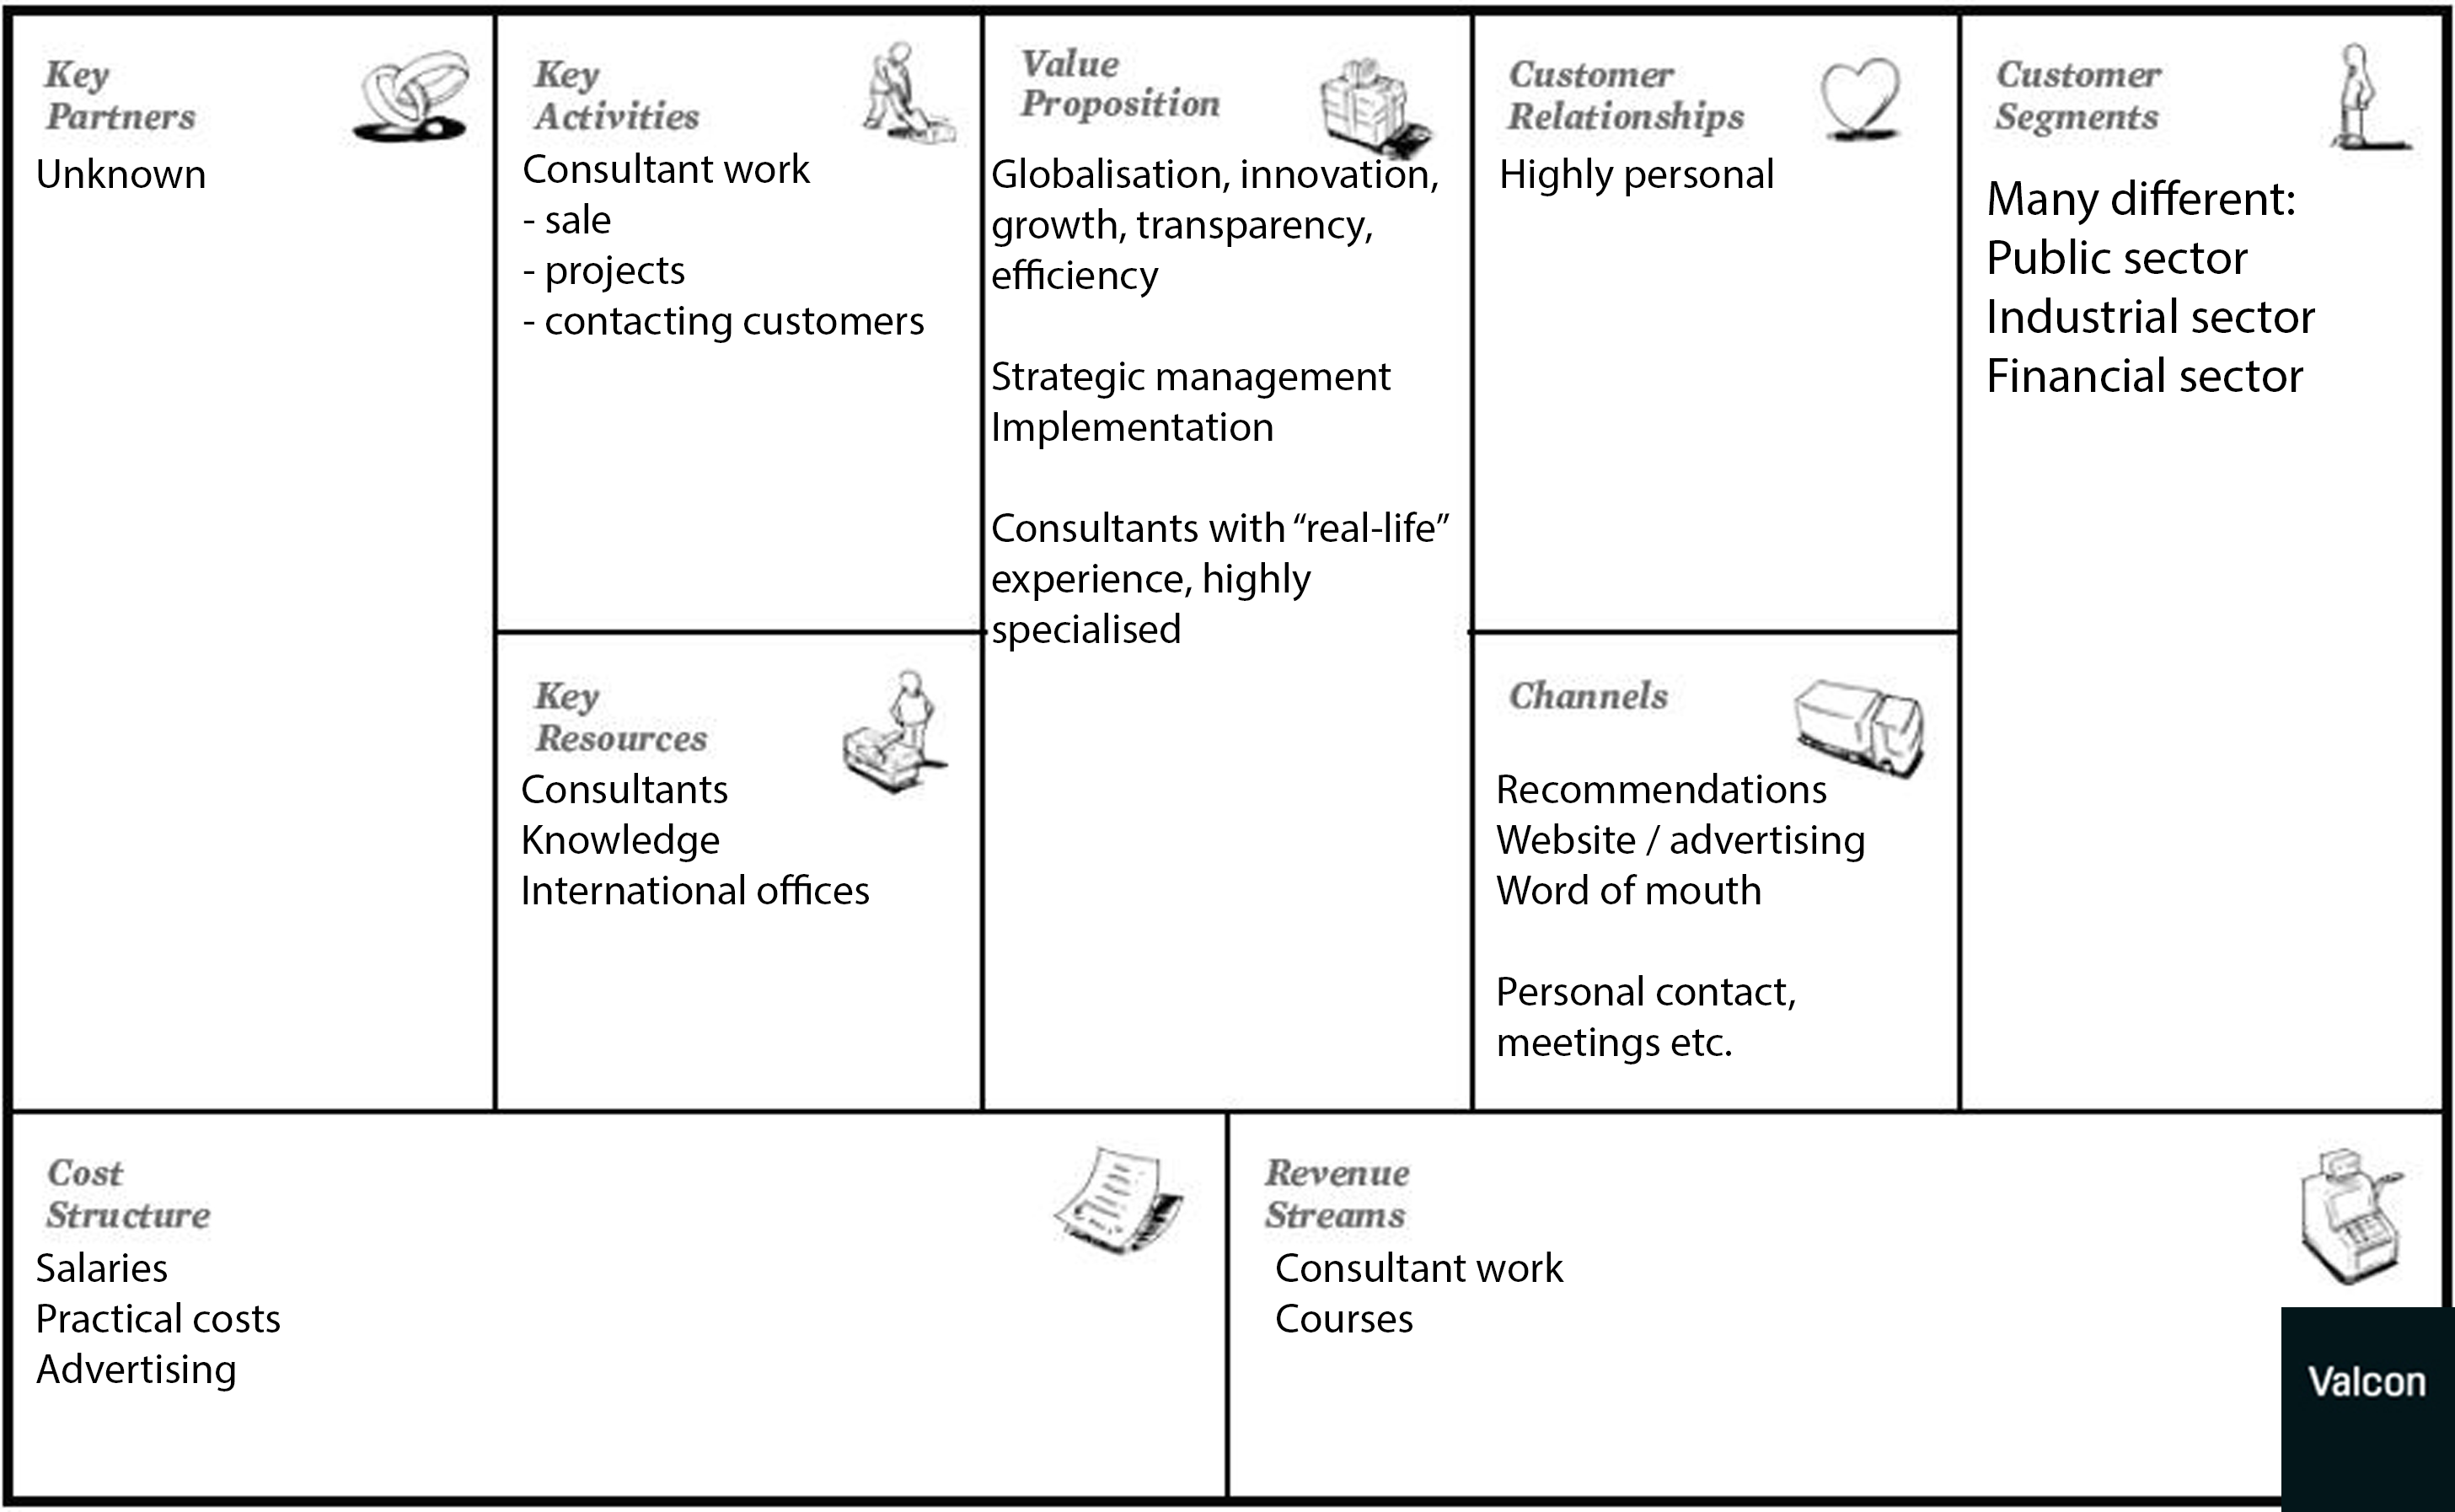
\includegraphics[width=\textwidth]{inline/business-model-canvas.png}
\caption{Valcon's business canvas.}
\label{fig:canvas}
\end{figure}

In relation to the problem it is important to note that the consultants are key resources for Valcon's business
as they are the ones who generate revenue.
As such it is important that they are able to perform their work effectively as soon as they start working at Valcon.
\section{Business strategy, IT strategy and company values}
\subsubsection{Business strategy}
We were not able to acquire Valcon's business strategy, as it is not public and Valcon were not interested in sharing it. (Source: Danni: "Det er korrekt at Valcon gruppens konkrete business strategi ikke er tilgængelig" (appendix \ref{app:business_strategy_refusal})). 
However, we were able to glean some of it through the interviews and meetings:

Valcon is in rapid growth and have a continued focus on keeping this growth as high as possible. 

(Sources: appendix \quoteref{app:danni_initiation}{danni_init_eksplosiv_vekst} and appendix \quoteref{app:danni_initiation}{danni_init_business_strategy_vekst}).

\subsubsection{IT strategy}
Valcon's IT strategy focuses on streamlining IT activities, being cost efficient, outsourcing labor intensive tasks, making work easier for the consultants, few but strong partnerships and choosing off-the-shelf systems instead of customized systems.

See appendix \ref{app:it_strategy} for the original document.

\subsubsection{Company values}
Valcon is guided by four values internally: Integrity, joy, performance, and competence.
Furthermore they value a flat hierarchy.
(Source: appendix \quoteref{app:danni_initiation}{danni_init_firmastruktur}).
\section{Work domains}
Entering newly hired employees into the systems at Valcon and requisitioning the required hardware is currently a stressful process.

Initiators of the process in both Valcon and OMT send information to accounting, who proceeds to enter information into some systems while IT enters information into other systems, sets the hardware for the new employee up, and sends it to him/her.
The new employee is contacted both by the initiators and IT, and sometimes by accounting as well.

But the core of the problem is that the process sometimes has to be very quick.
In that case, the initiators initiate the process both in IT and accounting at the same time, leading to more stress and intercommunication between them.

Looking at the process it seems essential to take a deeper look at the following work areas in order to get a better understanding of the problem:
\begin{itemize}
\item Recruitment (the initiators)
\item Accounting
\item IT
\end{itemize}

A visual representation of the organization as well as the work domains to research can be seen in appendix \ref{app:OrganizationalChart}
\section{Conclusion}
This section aims to explain how the recruitment process problem, we are dealing with, is relevant to Valcon as a whole.\\

\noindent Part of Valcon's business strategy is to keep a high growth rate for the company.
A high growth rate means many new employees.
All employments go through Group Support Functions (IT and accounting) in the recruitment process.
Group Support Functions has problems dealing with the current amount of employments.

Since Valcon intends to keep growing and Group Support Functions have problems keeping up, there is a need to optimize the process.
\chapter{In-depth analysis \\ Understanding the problem}
The following chapter will explain our approach to analyzing the process, describe the process in some detail and highlight key findings.

\section{Process analysis approach}
Based on the process analysis in which we identified the work areas relevant to the process, we conducted various interviews.
We chose to begin with interviewing Lisbeth (of accounting) and Peter (of IT), as they are the ones most affected by the process.
We chose to interview Hanne (NBA) as well, as she is the initiator of the process at Valcon.
Finally, we chose to observe both IT and accounting, to get a sense of the work flow there.

When we analyzed the data, we realized that we had to interview Jytte (process initiator at OMT) as well, as much of the problem originates in OMT.
\todo{Why no quantitative analysis? SOURCE}
\todo{Why no Valcon/OMT recruiter interview? SOURCE}
\section{Process description}
The process starts when a new employee has been hired.
An initiator (often Hanne or Jytte, sometimes other people) contacts accounting with information on the new employee.
A contract has to be formulated and, if there is information missing, the new employee has to be contacted in order to complete their particulars.

The information is entered into QHR and IT is contacted to let them know that a new employee has been hired.
IT then uses the information in QHR to create a new user in AD and give them a mailbox on the Exchange Server, and contacts accounting again with the employee's initials.
Accounting, after receiving the initials, enters the employee's particulars in Maconomy and Bluegarden (or in the case of foreign departments, the relevant salary system for that country).

At the same time IT contacts the new employee about their preferences for phone and internet.
When they have received these from the employee they contact Valcon's communications provider in order to set the new employee up according to their preferences.

Also at the same time, a PC is set up by IT according to the new employee's needs, based on which department they will work for.
Finally information about the handed out gear is recorded in TechAdm.

A visual representation of the process can be found in appendix \ref{app:ProcessChart}
\section{Key findings}
\subsection{Results from interviews}
There are several reasons why the current recruitment process needs to be optimized.

1. The main frustrations in the IT-department are that some recruitments occur with very short notice, and that data occasionally is incomplete.
(Appendix \completeref{app:peter} lines \lineref{peter_datamangel}, \lineref{peter_frustration1}, \lineref{peter_frustration2}, and \lineref{peter_frustration3})
The short notices are mainly rooted in recruitment of subcontractors in OMT, while the incomplete data occurs both with recruitments in Valcon and OMT.
(Appendix \quoteref{app:peter}{peter_short_notice})
Part of the problem with incomplete data is that the recruiters are not aware of exactly what information is needed in order to set a new employee up correctly.
(Appendix \quoteref{app:jytte}{jytte_stamdata})

We think that some of the frustration stems from IT not having a standard process for when data is incomplete.

2. The main frustration in Accounting is that employee data is managed in many different systems and needs to be copied manually.
(Appendix \quoteref{app:lisbeth}{lisbeth_manuelle_indtastninger})
Each employee in the recruitment process maintains their data on the new employees in individual spreadsheets.
(Appendix \quoteref{app:lisbeth}{lisbeth_ark})
This is problematic, as non-standard processes are hard to pass on.

3. A lot of time is spent communicating information back and forth between Accounting and Recruitment.
(Appendix \quoteref{app:lisbeth}{lisbeth_vende_tilbage})
Similarly time is spent communicating the information to the IT-department.
(Appendix \quoteref{app:lisbeth}{lisbeth_IT})
Accounting and IT want communication to be more standardized, while Recruitment finds it problematic because all data isn't necessarily available by the time of recruitment.
(Appendix \quoteref{app:lisbeth}{lisbeth_standardiseret_proces}, \quoteref{app:peter}{peter_standardiseret_proces} and \quoteref{app:hanne_interview}{hanne_ikke_standardiseret_proces})
Forcing standardized communication might put additional pressure on the consultant/manager in charge of the recruitment, which should be avoided.
(Source: appendix \quoteref{app:hanne_interview}{hanne_standardised})
At OMT, requiring standardized communication might be possible.
(Source: appendix \quoteref{app:jytte}{jytte_standardised})

With a common system for keeping the information, 2. and 3. could be avoided, as everyone could view the data within that system.

4. Time is spent on routine tasks, such as defining new initials.
(Appendix \quoteref{app:peter}{peter_initialer})
This could possibly be automated.

5. Time is wasted waiting for other employees, as IT doesn't have standard processes for communication.
(Appendix \quoteref{app:emails}{matias_on_structure})
This is outside our scope, but should be investigated.

A visual representation of the chain of problems can be found in appendix \ref{app:ProblemChain}.
A transcript of the interviews can be found in appendix \ref{app:interviews}.

\subsection{The numbers}
\begin{wrapfigure}{r}{0.5\textwidth}
\vspace{-20pt}
\centering
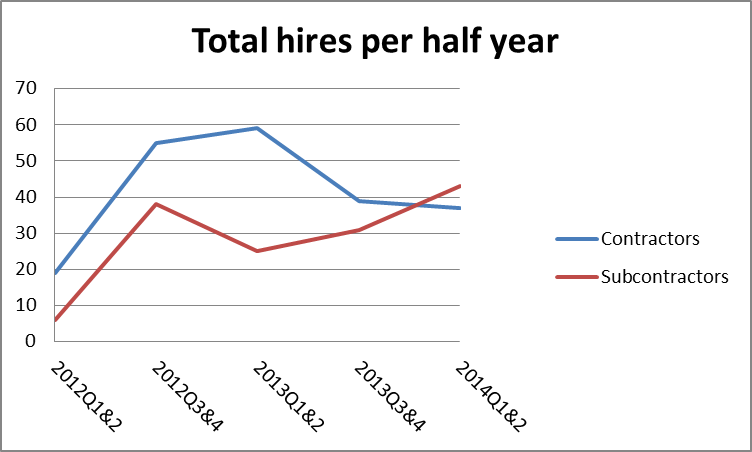
\includegraphics[width=0.45\textwidth]{appendix/total_hires_per_half_year.png}
\label{fig:total_hires_per_half_year}
%\caption{Total number of new hires per half year.}
\end{wrapfigure}
Looking at the number of new hires in Valcon we got an impression of the scope of the problem.
Even though there are some fluctuations there is a trend toward a growth in the number of hires.
This corresponds with the expressed business strategy of growth.
However, the data is not entirely conclusive, as we have only been able to look at the number of new hires within the last 30 months.
A table with all the numbers of new hires can be found in appendix \ref{app:recruitment_data} together with additional graphs.
\chapter{Innovation \\ Possible solutions}
In this section we will describe the most relevant solution propositions and, on the basis of a cost-benefit analysis, document the impact on the company as a whole.

\section{Solutions}
Please refer to appendix \ref{app:solution_propositions} (p. \pageref{app:solution_propositions}) for a complete list of solution propositions. Each solutions is listed with a verdict of its suitability, sorting out the most improbable.
The most relevant solutions are subject to cost/benefit analysis in the following sections. \todo{Implementation i hvert afsnit.}
\todo{Why no 1 solution but many?}

\subsection{Template for recruitment}
\emph{Description:} Create a template for recruitment so recruiters know what information is required. A template also functions as a checklist, ensuring that the writer knows what information to send.

\emph{Pros:} Could reduce the amount of missing information in the initial email to accounting or IT. 
Also leads to a better defined process.

\emph{Cons:} Requires additional work by recruiter. 
If template is too information heavy, some may ignore it.
Valcon employees dislike forms and rigid processes, so they may ignore it.

\subsubsection{Finance}

\subsubsection{Conclusion} Creating a template for OMT recruitment seems a good idea.
Creating one for Valcon would be a bad idea, as it would take time from management and consultants, but creating one for Hanne might work, as she would be reminded of the information required.

\subsection{Change of attitude toward IT}
\emph{Description:} Change the company attitude toward IT, from the current "they are there to fix my problems" to "they are there if I really need them".
We do not know how to implement this, but as Valcon is a consulting company, we assume they have a strategy for this case.

\emph{Pros:} May reduce the number of edge cases, recruiters would be more likely to send recruitment information in early or give warning that a quick recruitment is coming up.
Doesn't require extra time from recruiters.

\emph{Cons:} It would be hard to measure the success of the change - when is an attitude changed? - but measuring the result of the change could be done.

\subsubsection{Finance} For benefit, measure current number of edge cases and their average time cost.
Make a guess as to how many of these would be avoided with the change (15\%?).
Compute hours gained and multiply with wages for IT.
As for cost, 8-10 hours of work for a consultant might be enough to implement this.

\subsubsection{Conclusion} 

\subsection{Buffer of computers}
\emph{Description:} Keep 2-3 pre-installed computers ready for use at OMT and at Valcon, for emergencies or very quick recruitments.

\emph{Pros:} Would reduce response times to urgent recruitments.
Also useful if an employee's computer breaks, to reduce downtime.

\emph{Cons:} Needs a little more managing from IT, as
computers will need to be kept updated and ready.
As all computers are not in use, this creates a small overhead.

\subsubsection{Finance} Free. Benefit in time gained. Resources lying dormant.

\subsubsection{Conclusion}

\subsection{New HR system}
\emph{Description:} Acquire a new HR system to facilitate communication between accounting, IT, and recruiters.
Valcon is already looking at HR systems.

\emph{Pros:} Recruitment process becomes more standardized, as it always follows the same path.
Information becomes more consistent, as personal spreadsheets are less needed. 
This also safeguards against employees leaving.
Errors are less likely, as number of manual entries of information is reduced.

\emph{Cons:} Costly to implement, requires training of accounting, IT, and recruiter employees.
Also requires maintenance.

\subsubsection{Finance} +: Try to put a price on errors, count how many of them occur, guess how many will be eliminated, sum their costs.
Price of current HR system (Lotus Notes).

-: Price of new HR system.
Price of data transfer.
Price of training.
Price of maintenance.

\subsubsection{Conclusion} This solution is very necessary, as it is the only way information becomes more consistent.

\subsection{Other small improvements}

Write! \todo{The small improvements need including in the report.}

\section{Other recommendations}
Need rewriting \todo{Is this section good? Is it relevant?}

\subsection{Analyze OMT process}
Conduct an analysis of whether the OMT process can be improved so they know further in advance who and when someone is needed, so the number of urgent cases can be reduced.

\subsection{Further automation of install process}
The install process is very time consuming, and is a candidate for automation.
Looking into whether more of it could be automated could save time.


\appendix
\chapter{Glossary}
Particulars 	=	The core data of a person (name, address and more)
Lotus Notes		=	Platform at which QHR and TechAdm is hosted	\\
QHR				=	HR platform used to store information about new employees	\\
AD				=	Active directory. Platform used to generate and organize information in the Valcon portal, user control and permissions	\\
TechAdm			=	Platform used to store information about rented hardware	\\
Maconomy		=	Platform used to administrate invoices	\\
Exchange		=	Platform used to administrate the Valcon mail system	\\
BlueGarden		=	Platform used to administrate salaries in Valcon Denmark	\\
\chapter{Project Agreement}
\section{Premise}

\subsection{Background}
In Valcon, the process of registering new employees is characterized by loose organization. This is a problem, as the company is growing quickly and many employees are recruited, and specialists are recruited for short periods of time. We have been asked to research this process and explore possible solutions, and finally to write a business case explaining the benefits and drawbacks of different solutions.

\subsection{Assignment and Objective}
The objective of the project is to research the process of registering new employees. HR departments in both OMT and Valcon collect information on the new employee and send this to either an accountant or the IT department, depending on what they need done first. This creates an unnecessary need for communication between the IT department and the accountant, which might be avoided if the process was standardized. The accountant enters financial and personal information into a system (QHR), which the IT department then uses to send a computer, setup internet connection and phone accounts, and enter the employee into the central system (AD). To further understand the current situation, the project group will conduct an ethnographic analysis of the process, in an attempt to discover parts of the process that could be effectivised, and look at ways to do so.

\subsection{Financial framework}
There will be no money involved in the project.
The resulting report of the project may be used freely by Valcon.

\subsection{Critical factors}
\textbf{Success factors:}
The solutions proposed should reduce the time, complexity and effort it takes to enter a new employee into the system.
The Business Case provided by the group must, regardless of the solutions proposed, be useable as documentation for the existence of the problem.
The solution proposed must still make use of the Active Directory which Valcon uses for managing their IT structure.
\textbf{Critical preconditions:}
We need to be able to get the time needed from the resources mentioned below.

\section{Organization}
\subsection{Project organization}
The project organization consists of two groups. The project group at ITU consists of Michael Frikke Madsen, Jonas Kastberg Hinrichsen, Martin Juul Petersen, Jakob Ambeck Vase, and Jakob Merrild. They report to Danni Jensen at Valcon.

\subsection{Resources}
The time of the project group.
3 meetings (with a 4th optional one) with Danni Jensen of appr. 1 hour each.
One or two interviews with each key employee in the process (Lisbeth, Peter, Mathias, HR) of appr. 30 min. each.
Open doors, for observing the work practises involved in the process.

\subsection{Stakeholders}
Danni Jensen
Lisbeth Justesen
The IT department of Valcon
HR departments of OMT and Valcon

\subsection{Agreements}
The following agreements were made:
The project group can conduct observations of public areas at Valcon without prior notice.
In order to conduct interviews with and observations of individuals, an agreement must be made with Danni Jensen, who must authorize the project group to initiate contact with the person to be interviewed. 
After the initial contact has been made, the project group is free to contact the person directly in order to make an appointment.

\section{Method}
\subsection{Overall Approach}
The overall approach to the project will be using the MUST method. The MUST method consists of the following four phases:
Initiation phase, where we agree on the problem and a contract
In-Line analysis, where the project group will align the project’s goals with the company’s IT and business strategy
In-depth analysis, where the project group will observe and document the relevant work practices
Innovation phase, where solutions will be investigated and optionally presented

\subsection{Plan}
\begin{itemize}
\item[13/10] - End of In-Line phase.
\item[15/10] - Meeting after In-Line and before In-Depth phases.
\item[10/11] - End of In-Depth phase.
\item[14/11] - Meeting after In-Depth and before Innovation phases.
\item[4/12] - End of Innovation phase
\item[Before] 17/12 - Delivery of Business Case
\item[??] - Optional meeting after Innovation phase.
\end{itemize}

\subsection{Signatures}
\chapter{Problem Statement}
\label{app:problem_statement}
How can the Valcon Group save time and reduce frustration in the IT and Accounting departments by improving the process of new employee registration?
\\\\
Specifically:
\begin{itemize}
\item How can they reduce redundant work?
\item How can they automize routine tasks?
\item How can they reduce the amount of cases not following the standardized process, or refit the standardized process to accomodate the open structure of the company?
\end{itemize}

The following requirements need to be fulfilled for the project to be considered a success:
\begin{itemize}
\item
We must document the process to prove that there is a problem.
\begin{itemize}
\item If we prove that there is a problem, this requirement is fulfilled.
\end{itemize} 
\item
Having a standardized process reduces frustration and saves time, therefore communication should go through accounting every time, or standard process should be changed to allow for multiple paths.
\begin{itemize}
\item
Measure the amount of tasks currently not following standard process (mean/month)
\item
After implementation, measure the amount of tasks not following standard process (mean/month)
\item
If the number of tasks not following standard process after implementation is reduced by 50\%, this requirement is fulfilled.
\end{itemize}
\item
Tasks that could be automated, should be.
\begin{itemize}
\item
Look at the process, find all the tasks that could be automated and the ones that already are, make a list stating whether a task is manual or automated, and whether it must be manual or could be automated.
\item
After implementation, look at the list and compare the number of “could be automated” tasks to current process.
\item
If 50\% of the tasks that were previously not automated, but could be, are now automated, this requirement is fulfilled.
\end{itemize}
\item
The current speed of the process must be maintained or improved.
\begin{itemize}
\item
Measure the current mean time from first mail to accounting or IT, to employee is registered and IT tasks are done before and after implementation.
\item
If this time is the same or (preferably) faster, this requirement is fulfilled.
\end{itemize}
\end{itemize}
\chapter{Valcon environment}
\label{app:valcon_environment}
Valcon operates within an competitive environment where image and contacts are key. 
There's a great need for experienced and knowledgeable consultants but there's also a lot of competition in the field.
Not because there are a lot of competitors within the fields that Valcon works in, but rather because the competitors are the same every time.
This means they know each other and know exactly what kind of prices and quality the opposing firms will bring.
Due to this, Valcon's business strategy has been to hire the best and brightest employees and accept the fact that they're unable to be the cheapest organisation to hire.

They sell themselves mainly on knowledge and quality, rather than on price and pride themselves on being a company capable of the entire consultation process, from analysis to implementation.

They refer to themselves as the 'how' company, as they are often employed in projects where a competing consultation firm has been hired to write the analysis report and figure out 'what' to do. 
Valcon are then employed to conclude the project by implementing the solution.

Valcon's biggest threat is losing their consultants.
Consultants are drawn towards new and exciting opportunities, while working for the same company for a long time gets increasingly stale.
This means that sooner or later a consultant will grow tired of the current challenges he's facing and move on to another company.

For references, see \completeref{app:danni_initiation}, \completeref{app:danni_inline} and the Valcon website.
\chapter{OMT environment}
\label{app:omt_environment}
OMT operates within an environment where they aren't facing a lot of competition. 
There aren't many firms designing war ships, and this places OMT in a favorable position.

There aren't many ship designers with experience on war ships, so when OMT needs employees there aren't many candidates, and most of them are already employed elsewhere.
Because of this, OMT hires a lot of their workforce within other ship design companies.
Since these companies work in other fields than OMT, they usually don't mind subcontracting the employees that OMT needs, as this gives them more money. 
\chapter{Valcon Business Canvas}
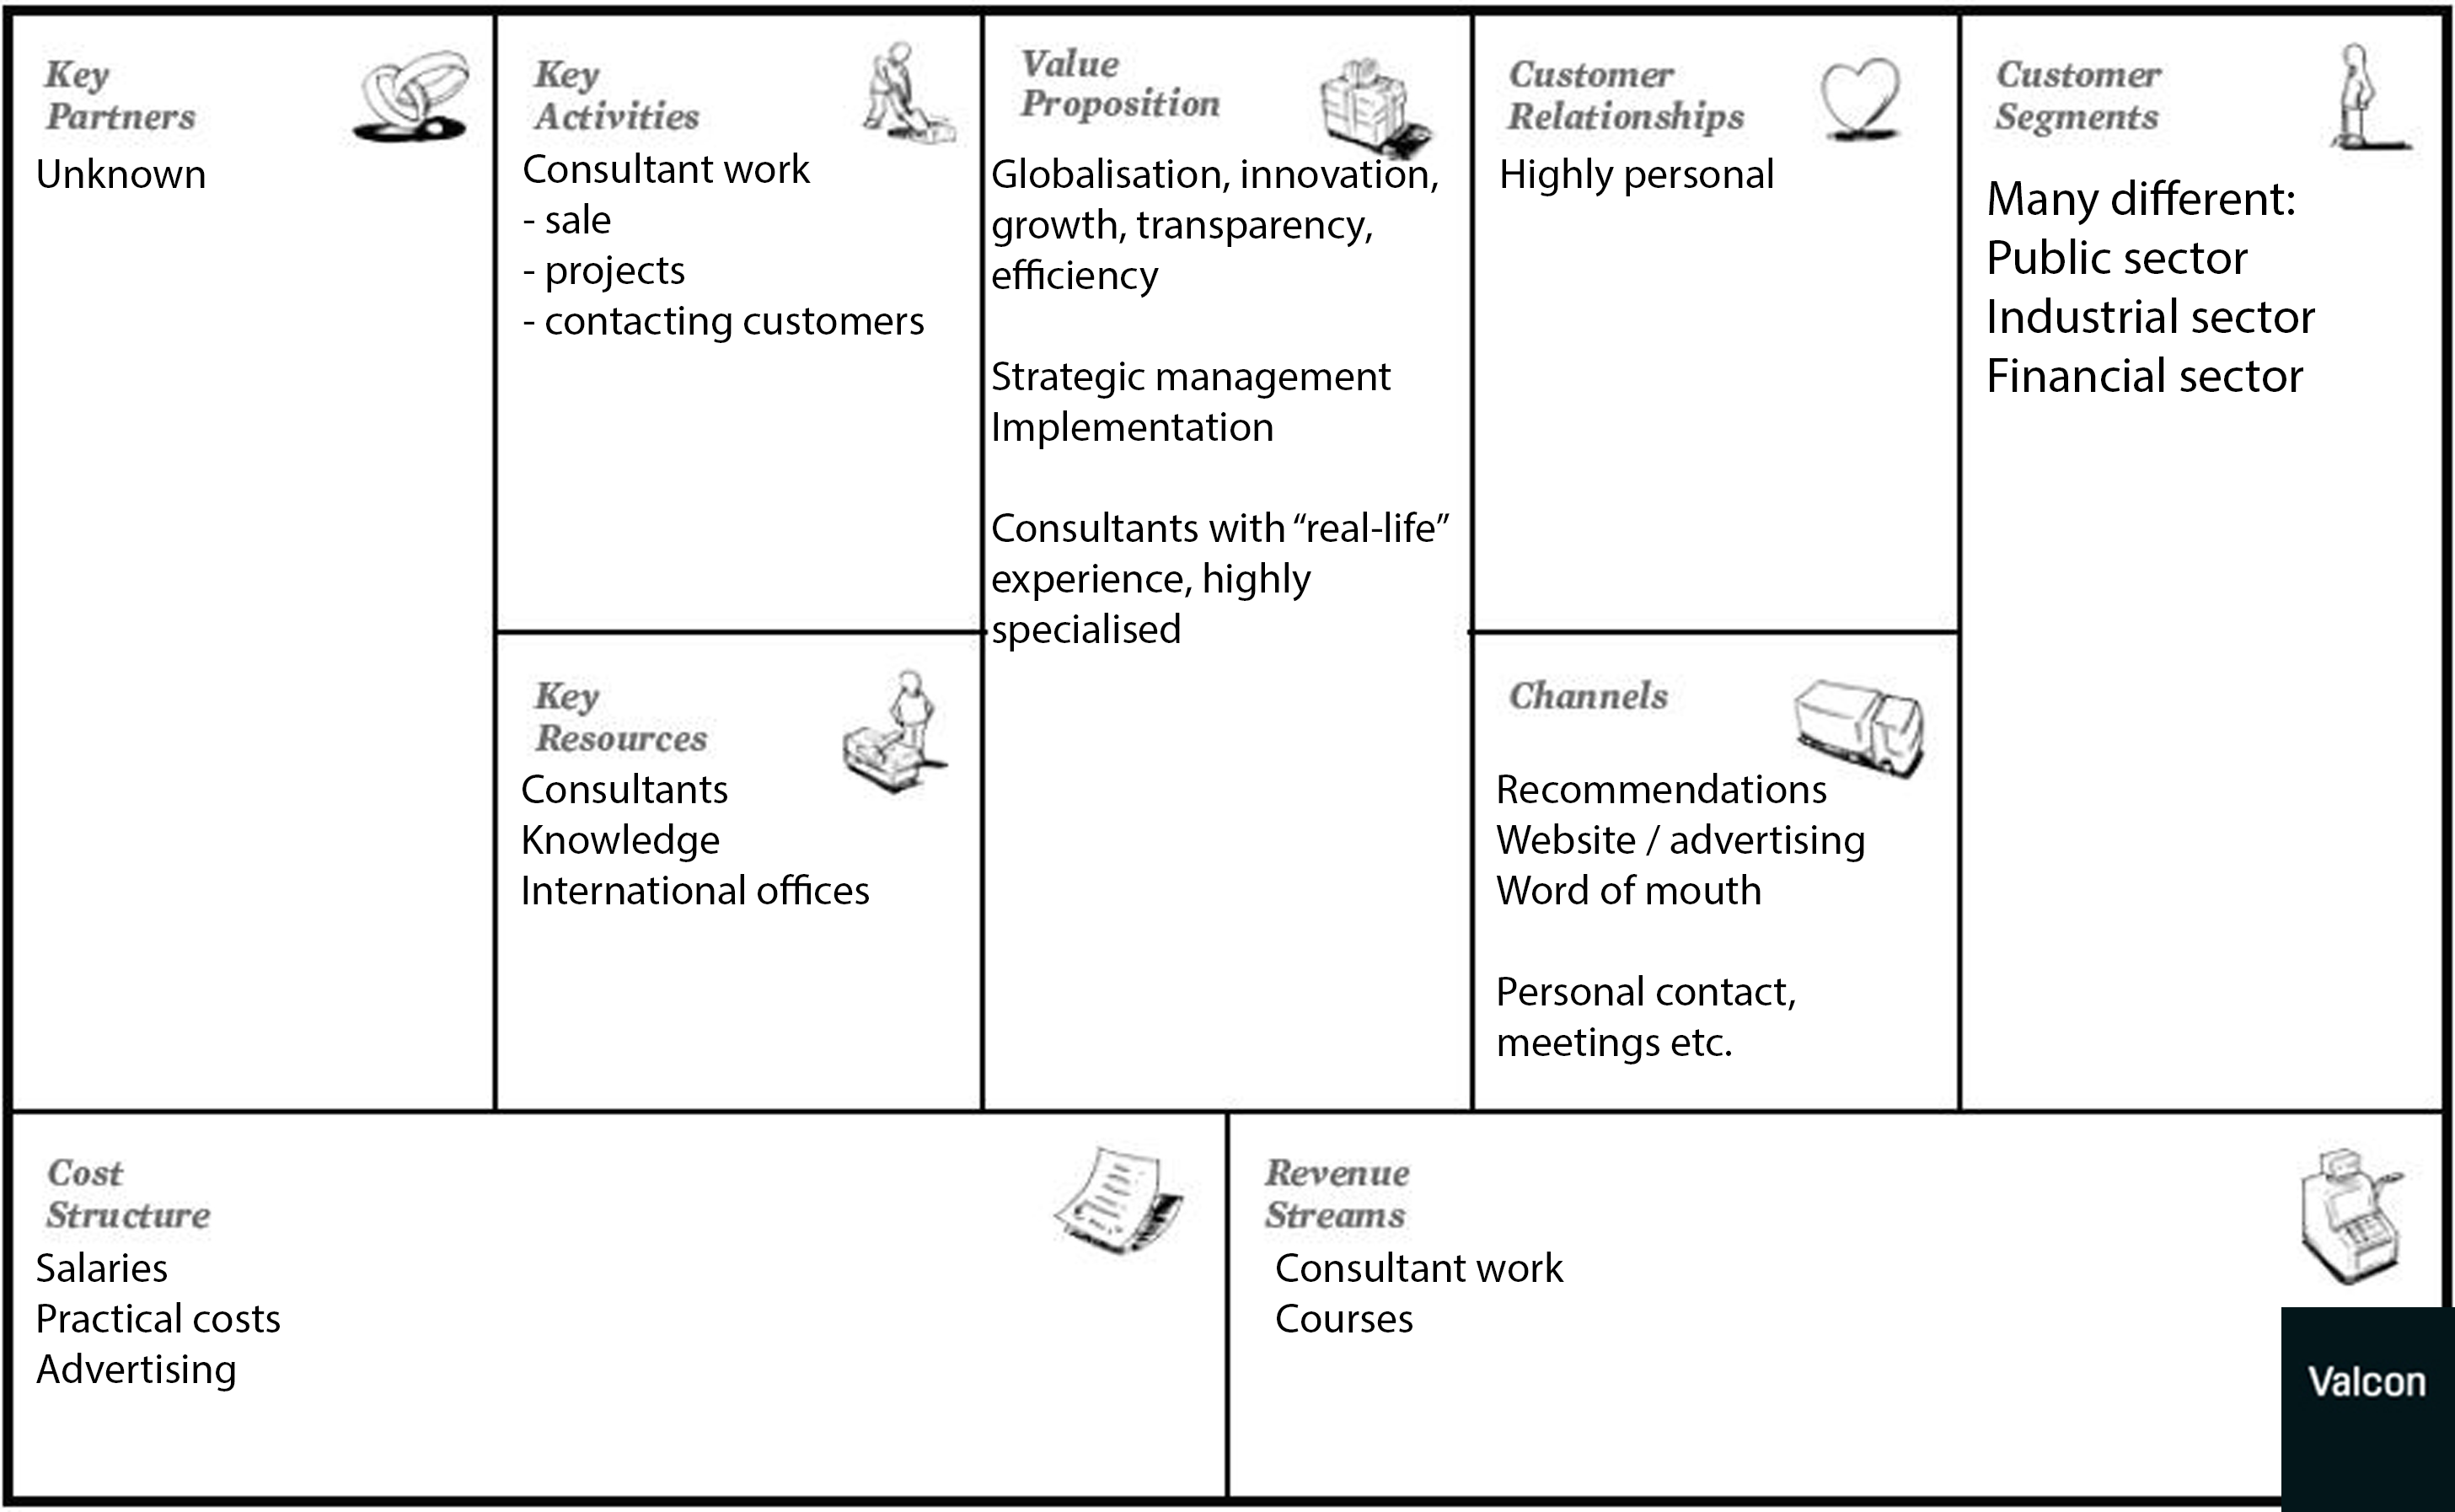
\includegraphics[angle=90,height=475pt]{inline/business-model-canvas.png}

The business canvas gives an overview of Valcon as a business - what services they provide, what their key resources are and so on.
We constructed the canvas primarily from information from the Valcon website, along with information from initial interviews with the IT Manager of the company.
The canvas was later presented to the IT Manager, and then refined slightly from his feedback.

\includepdf[pages={1-2},pagecommand=\chapter{Valcon's IT strategy},scale=0.75,nup=1x2]{appendix/it_strategy.pdf}
\label{app:it_strategy}

\includepdf[pages={3-},scale=0.75,nup=1x2]{appendix/it_strategy.pdf}
\chapter{Organizational Chart}
\label{app:OrganizationalChart}
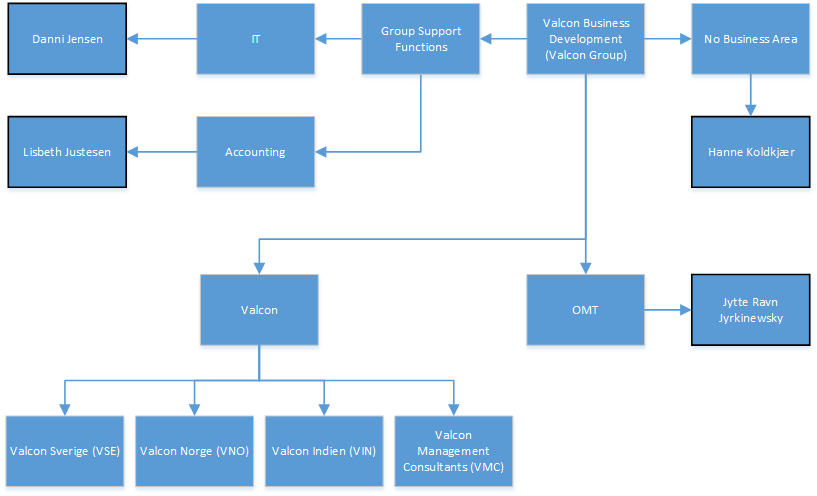
\includegraphics[angle=90,height=475pt]{appendix/organizational_chart.png}

\chapter{Process Chart}
\label{app:ProcessChart}

This chart visualises the process.\\\\

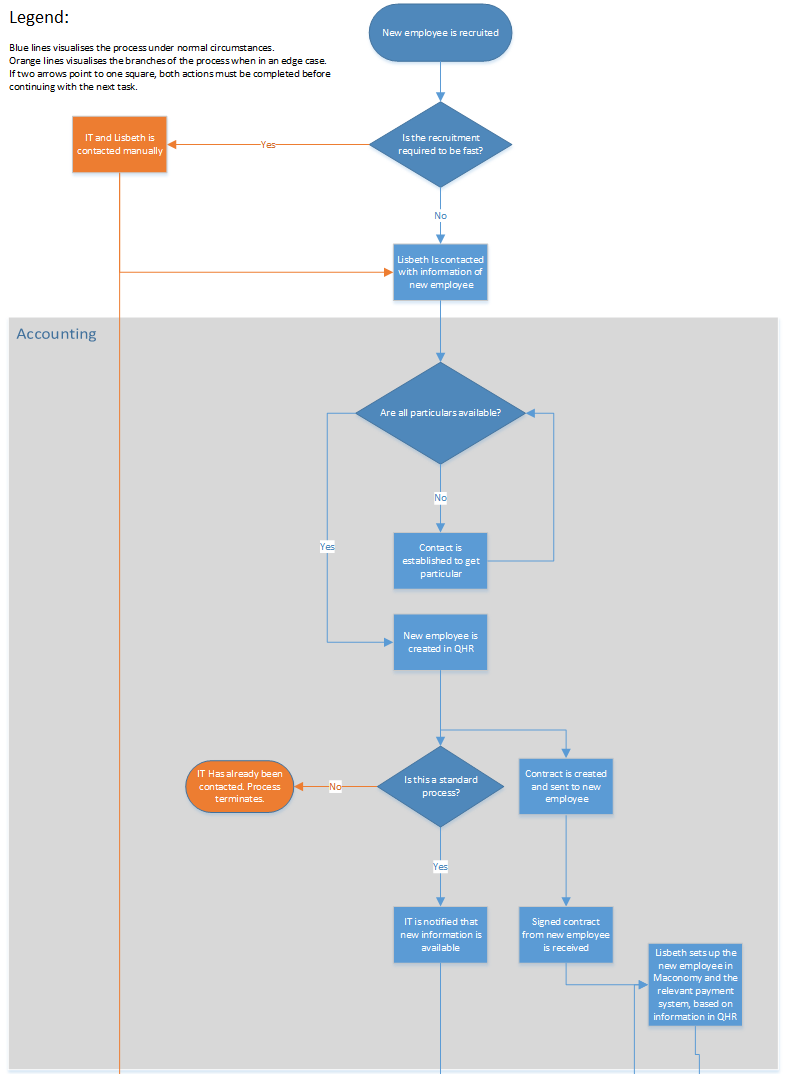
\includegraphics[scale=0.65]{appendix/ProcessFlowChart1.png}

\newpage

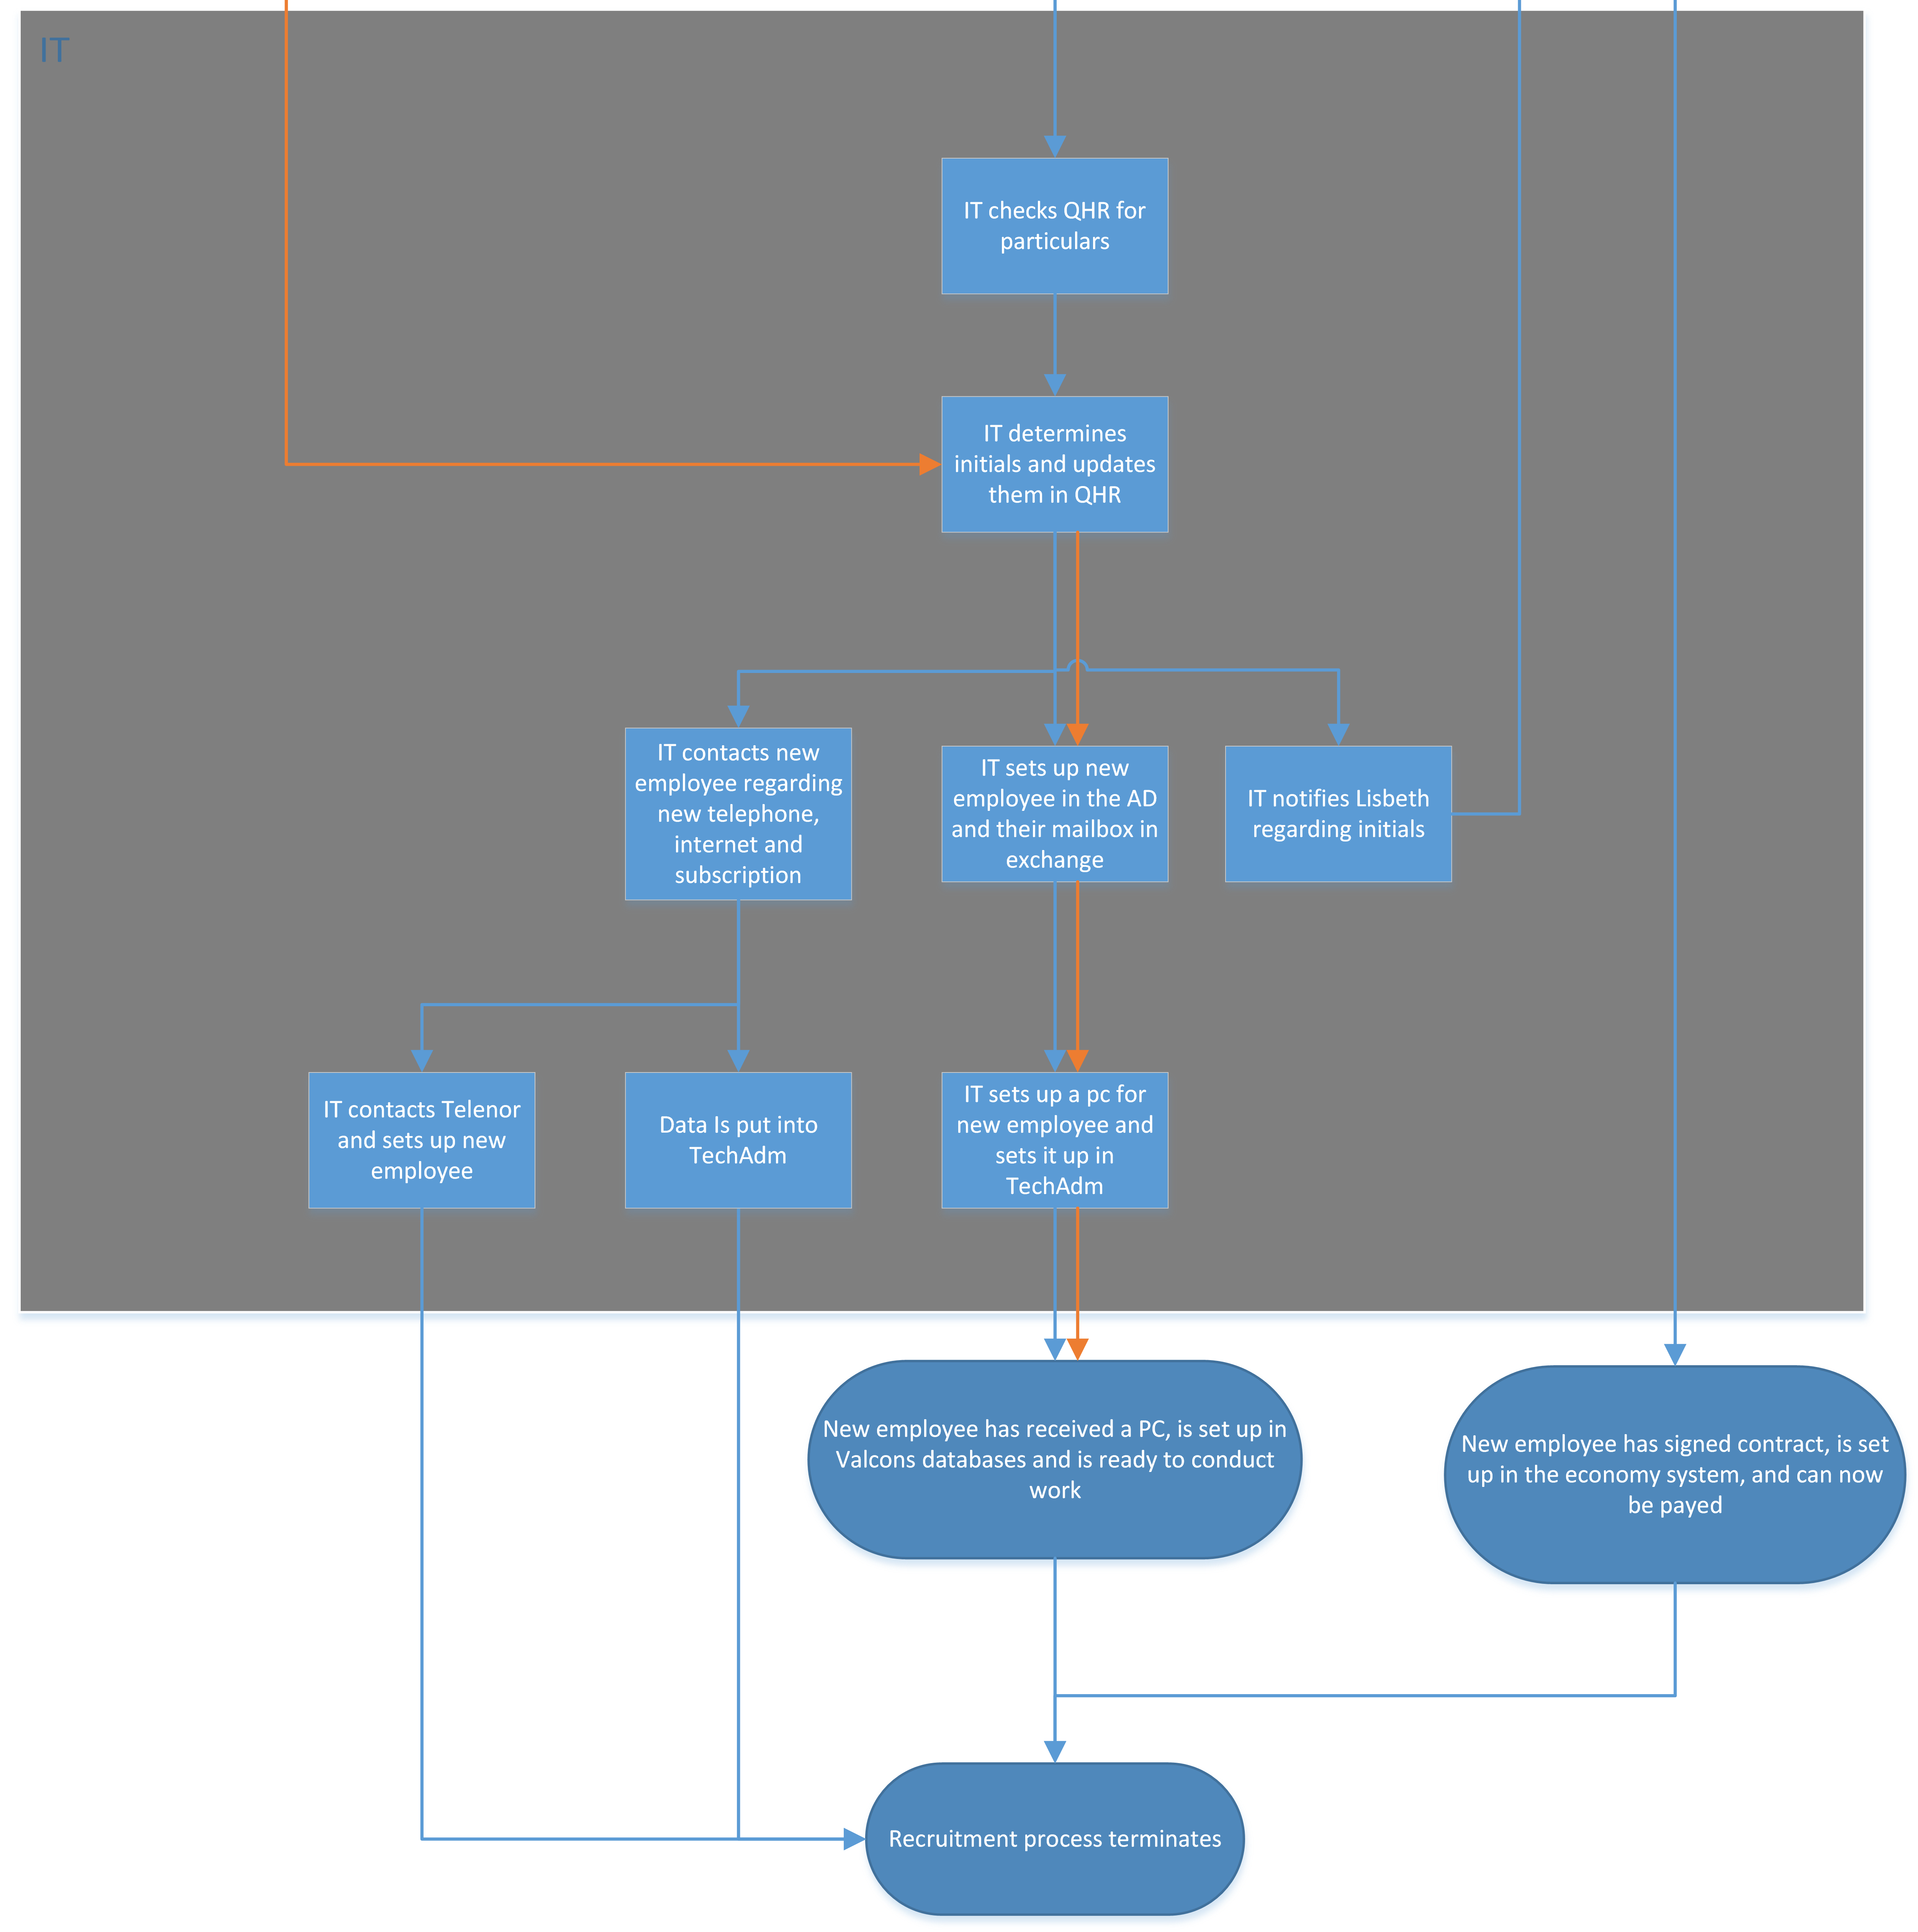
\includegraphics[scale=0.65]{appendix/ProcessFlowChart2.png}
\chapter{Problem Chain}
\label{app:ProblemChain}

Problem chain visualizing the origin of each problem.

If a problem's reason points to another problem, then that problem is what must be fixed.
The reasons that do not point to other problems are the ones that we wish to fix with our solutions.
\\\\

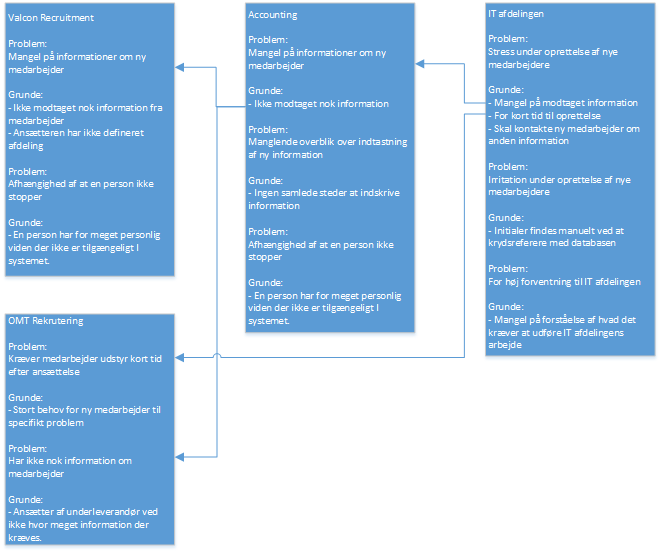
\includegraphics[width=\textwidth]{appendix/ProblemChain.png}
\chapter{Solution propositions}
\label{app:solution_propositions}
\section{List of proposed solutions}
\begin{enumerate}
\item Software that does it all
\item Template for recruitment
\item Adjust expectations between IT and Valcon
\item Buffer of ready computers
\item Increase IT staff size
\item New HR-system
\item Help-program for finding initials and reading templates
	\item Other small improvements
	\begin{enumerate}
	\item Phone and internet paper in contract letter
	\item "Unkown department" in IT-systems
	\item Mail from OMT when recruitment is assured, but data is not yet available
	\end{enumerate}
\end{enumerate}

\section{Explanation of solutions}
\subsection{Software that does it all}
\emph{Description:} This proposal is for a piece of software that can encompass all the requirements of every employee in the company. Lotus Notes had this status once, but many disliked it.

\emph{Origin:}
When interviewing the accounting department it was noted that such a system would help out with a lot of the prevalent tasks.
(Source: appendix \quoteref{app:lisbeth}{lisbeth_system})

\noindent \emph{Pros:} Only one place for information, easy to manage.

\noindent \emph{Cons:} Very expensive, very hard to accomodate everybody.

\emph {Verdict:}
Not suitable. The solution is in direct opposition to the business strategy of the company, as it would require a large amount of concrete templates, training and time on behalf of the consultants.

\subsection{Template for recruitment}
\emph{Description:} When a new recruitment process starts, instead of a mail being sent with the information, a template is used to ensure that no information is missing.

\emph{Origin:}
In various interviews it was mentioned how lack of information damaged the recruitment process a lot, by increasing the overall work load required.
(Source: appendix \quoteref{app:lisbeth}{lisbeth_vende_tilbage} and appendix \quoteref{app:peter}{peter_information})

\noindent \emph{Pros:} No information missing means no need to contact employee more than once, saving time.

\noindent \emph{Cons:} Will put more work on recruiter, and Hanne stated that employees at Valcon dislike templates, so they won't use them.

\emph{Verdict:}
Partially suitable. The solution is in direct opposition with the Valcon business strategy, and thus we would not recommend it. However, based on interviews with the OMT partition of the company, templates would be possible for recruitments on their end. Thus we recommend it for the OMT group.

\subsection{Adjust expectations between IT and Valcon}
\emph{Description:} Currently, IT is generally regarded as a department that just solves whatever problem one might have. Some employees in the IT department do not agree. Adjusting the expectations between the IT department and Valcon could have benefits.

\emph{Origin:}
When interviewing the IT department there was a notion that the company did not realise the amount of effort put into the work of the IT department, nor did most understand how complicated it was if recruitment requests were admitted with little to no spare time.
(Source: appendix \quoteref{app:peter}{peter_frustration3})

The other interviews backed up this notion, as they seemed to not know the implications of the IT department's work processes.
(Source: appendix \quoteref{app:lisbeth}{hanne_omIT} and appendix \quoteref{app:hanne_interview}{hanne_losningomIT})

\noindent \emph{Pros:}
If people are more aware of how the IT department functions, they are more likely to be considerate. If the IT department are more aware of how Valcon functions, they will better understand why their work is critical. This would improve job satisfaction.

\noindent \emph{Cons:} Hard to implement, hard to measure.

\emph{Verdict:}
Suitable. In order to maintain a high satisfaction for all employees, it is important that everyone understands each others work loads, and how it is increased under certain conditions. It could be achieved through generic information channels in the company.

\subsection{Buffer of ready computers}
\emph{Description:} Have a few number of computers installed and ready for use at Valcon and OMT.

\emph{Origin:}
In various interviews it was mentioned how this solution could ease the overall process, as it can deal with the situation of a critical recruitment.
(Sources: \quoteref{app:hanne_interview}{hanne_buffer} and \quoteref{app:jytte}{jytte_buffer})

\noindent \emph{Pros:} Better response times to urgent recruitments. Useful if an employee's computer breaks at a critical time.

\noindent \emph{Cons:} Needs a little more managing from IT, and maybe a full time IT employee at OMT. Computers will need to be updated. Resources not in use.

\emph{Verdict:}
Suitable. Having a buffer of computers would increase overall budget, but would solve many issues related to the recruitment process.

\subsection{Increase IT staff size}
\emph{Description:} Increase the IT staff size to increase throughput.

\emph{Origin:}
Baseline solution

\noindent \emph{Pros:} Makes IT capable of doing more.

\noindent \emph{Cons:} Expensive, and management increases.

\emph{Verdict:}
Not suitable. Simply increasing the size of the IT staff to accomodate demand is not a proper solution, as it would not increase the amount of capable workers. This is due to increased management of the IT department. The issues faced in the process cannot be reduced by simply having more employees working on it.

\subsection{New HR system}
\emph{Description:} Implement a new HR system for communication between accounting and employers.

Valcon are already looking at new HR systems.

\emph{Origin:}
In the interview with accounting, it was mentioned how the current HR system was deprecated, and not very user-friendly.
(\quoteref{app:lisbeth}{lisbeth_HR})
A new HR system would help the process in a way, that information has to be typed in fewer times.

\noindent \emph{Pros:} Process becomes more standardized and information more consistent. Copying data fewer times reduces probability of errors.

\noindent \emph{Cons:} Costly and requires training.

\emph{Verdict:}
Suitable. A new HR system would affect the company positively in relation to their business strategy.

\subsection{Help-program for finding initials and reading templates}
\emph{Description:} 
Write a small program that can read the template proposed above and enter the information into the IT systems.
Also able to propose initials for employees, and check whether the exchange mailbox has been used before.
Would reduce workload for IT and introduce fewer errors, but would require some maintenance and some time initially.

\emph{Origin:}
When interviewing the IT department it was mentioned how a tedious task it was to make up new initials. Since the making of initials are based on certain rules it is possible to generate them automatically. Furthermore they have to input data in various databases, as well as updating possible deprecated data.
(Sources: \quoteref{app:peter}{peter_initialer} and \quoteref{app:peter}{peter_old_employees})

\noindent \emph{Pros:} 
Less time used to making initials. Reduction of tedious tasks that must be conducted often.
Less time used on inputting data, reduction of possible typing errors.

\noindent \emph{Cons:} 
Generated initials might form unsuitable words, and the process has to be overridden by the employee.
System might be insufficient and not be capable of handling deprecated data correctly. 

\emph{Verdict:}
Partially suitable. The initials systems can be implement fairly easy. It can be taken into account that it must be possible to manually input initials if the generated initials are not sufficient.
The automated system will be too difficult to manage.

\subsection{Other small improvements}
\begin{itemize}
	\item Phone and internet paper in contract letter\\
	
			Put a paper in the contract letter sent to new employees, asking for their internet and phone preferences. Give it to IT upon return. Would help reduce missing data for new employees, and save time in IT.
			(Source: \quoteref{app:peter}{peter_blanket})			
	
	\item "Unkown department" in IT-systems\\
	
			Create a department for unknown departments in the IT systems, possibly both for Valcon and OMT, and create a process for managing it.
			Would remove the department requirement from IT, allowing for quicker recruitment.
			(Source: \quoteref{app:peter}{peter_datamangel})
			
	\item Mail from OMT when recruitment is assured, but data is not yet available\\
	
			Have OMT write a mail to IT when they know they will hire an employee soon, but don't have the data yet, so IT can plan accordingly.
			Would reduce stress, but increase planning for OMT.
\end{itemize}
\chapter{Cost-benefit analysis}
\label{app:cost_benefit_analysis}
These calculations are based on the recruitment and resignation data sheet in appendix \ref{app:recruitment_data}.

\section{Standard process and edge cases}
\begin{itemize}
\item In 2012/13, 118 persons were hired or subcontracted.
\item In 2013/14, 154 persons were hired or subcontracted.
\item In 2014/15, 80 persons have been hired or subcontracted so far.
\end{itemize}
These numbers show how many computers have been made ready by year.
\emph{There is a small increase in the number of computers being readied (30\% in 2013 and (projected) 4\% in 2014).}

\subsubsection{Time spent on computers and data entering}
Peter gave an estimate for how long it took him to set up a computer and enter data into the system, 45 minutes (appendix \quoteref{app:peter}{peter_estimat_setup}). (We realize Peter may be wrong about this. We haven't been able to observe the process, but we still think the calculations are useful.)

Similarly, Lisbeth estimates that she spends about 15 minutes entering data into the system. (appendix \quoteref{app:lisbeth}{lisbeth_time_spent})

This means, that 118 hours have been used in 2012/13, 154 hours in 2013/14, and 80 hours in 2014/15 so far on computer setup and data entering.

With about 150 hours used every year, even if we save 30 minutes for every recruitment, this is only 75 hours saved every year, so \emph{our proposed solutions need to be inexpensive.}

\subsubsection{Time spent on other things related to recruitment}
Peter uses time on gathering information on telephone and internet connection preferences from the new employees, appr. 10 minutes on average.
(appendix \quoteref{app:peter}{peter_estimat_contact})
This is only on the Danish recruitments, and not on subcontractors.

Furthermore, he uses time on Danish resignations, both subcontractors and hires, appr. 15 minutes on average.
\todo{Where do we know this from? We dont know this from anywhere = picnic}
(We realize Peter may be wrong about these. We haven't been able to observe the process, but we still think the calculations are useful.)

\todo{Write something about Lisbeth spending time on acquiring information in edge cases?}

\subsubsection{Total time spent}
Here follows the total amount of time spent on recruitments and resignations each year (barring edge cases).
\begin{itemize}
\item 2012/13 - 140,5 hours.
\item 2013/14 - 186,5 hours.
\item 2014/15 - 95 hours so far. (Half the year has passed, so a reasonable estimate is that 190 hours will be used in total.)
\end{itemize}

As long as there are few edge cases, \emph{the time spent is a small problem.}

\subsubsection{Edge cases}
We haven't been able to get any numbers on the amount of edge cases in the process.

This is problematic, as our main focus is documenting that there is a problem, and the amount of time used without edge cases is small.

And even when edge cases happen, as the process doesn't change, \emph{the time spent doesn't increase, only the amount of frustration in the IT department.}

\subsubsection{Benefits to improving the process}
There are some benefits to changing the recruitment setup process.

Currently, IT and accounting are both frustrated by the process.
By improving the process, the work enjoyment could improve.

Finally, improving the process can speed up response times on support and recruitment from IT and on recruitment in accounting.

\subsubsection{Conclusion of process analysis}
There is little financial gain in changing the recruitment setup process.

The benefits, however, are important and in line with the Valcon's employee values.

So the solutions we propose must be without or with very little cost.

\section{Cost/benefit of solutions}
In this section, we look at the costs of each of our proposed solutions and write a few benefits.
We will not look at the new HR system, as Valcon is already working on it and we do not know enough about the system to correctly estimate costs and benefits. \todo{maybe remove}
To see a description of the solutions, see appendix \ref{app:solution_propositions}

\subsubsection{Software that does it all}
\begin{itemize}
\item \emph{Costs} - Very high. (\textgreater 1,000,000 DKK, drawing on comparable IT solutions in other companies.)
\item \emph{Benefits} - Accounting and IT would be happy, as all data would have to only be entered once. But consultants would be less so, as their work would be slowed down by data entering and a heavy program. (Lower income.)
\item \emph{Conclusion} - This investment would never break even.
\end{itemize}

\subsubsection{Template for recruitment}
\begin{itemize}
\item \emph{Costs} - Three hours for creating the template, an hour every six months to keep it up to date. (500 * 3 = 1500 DKK initially, 500 * 2 = 1000 DKK annually. (Assuming 500 DKK/hour for the employee making and maintaining the template.))
\item \emph{Benefits} - Lisbeth saves time, as data isn't missing, but Hanne and Jytte spend a little more time gathering the information. All three save time as less communication between them is needed. (Lisbeth saves appr. 10 minutes per recruitment, Hanne goes even, Jytte goes even.) (Minutes saved * number of recruitals annually / 60 = hours saved annually = 10 * 180 / 60 = 30 hours saved annually = 9000 DKK saved annually (assuming 300 DKK/hour))
\item \emph{Conclusion} - This investment would break even in the first year, even saving 6500 DKK, and would save 8000 DKK annually afterwards.
\end{itemize}

\subsubsection{Change of attitude toward IT}
\begin{itemize}
\item \emph{Costs} - (Example:) A small, internal campaign to change company attitude might cost appr. 20,000 DKK (Two days work for a designer, printing posters, sending emails, lost time for consultants).
\item \emph{Benefits} - Better communication with IT. We cannot see any financial gain. Would reduce frustration in IT and make IT feel more appreciated.
\item \emph{Conclusion} - Won't break even, but the non-financial benefits are important.
\end{itemize}

\subsubsection{Buffer of ready computers}
\begin{itemize}
	\item \emph{Costs} - 240,000 DKK initially (20,000 DKK * 12 computers). Appr. 1,200 DKK annually for maintenance (8 hours work for a student-helper, 150 DKK per hour pay.)
	\item \emph{Benefits} - Shorter response times from IT, less frustration in IT. Time saved in IT as the computers can be created at the same time. 96 hours saved by student helpers annually = 14,400 DKK saved annually. In cases where a quickly hired employee would not normally be able to start work, because of a delay in getting them a computer, having a buffer can potentially save a lot of money.
	\item \emph{Conclusion} - Will break even after less than 18 years, potentially faster if there are a couple of cases of lost workdays per year. Less frustration in IT and better response times make it worth it.
\end{itemize}

\subsubsection{Increase IT staff size}
\begin{itemize}
	\item \emph{Costs} - Appr. 1,000,000 DKK annually. (Full time employee + management and resource costs.)
	\item \emph{Benefits} - Less frustration in IT. IT would be able to handle a higher workload generally, not just with regards to the process of new employee registration.
	\item \emph{Conclusion} - This is a very expensive solution to the problem. 
\end{itemize}

\subsubsection{New HR-system}
\begin{itemize}
	\item \emph{Costs} - Because the Valcon Group is already looking into a new HR-system it doesn't seem necessary to look at the costs.
	\item \emph{Benefits} - Assuming that the Recruitment, Accounting and IT departments would all be able to access shared information within the new system a total of approx. 60 minutes can be saved per hire across departments. With about 150 new hires per year, a total of 150 hours can be saved. Assuming an average cost of 500 DKK per work hour this is equivalent to 75,000 DKK. (Sources: Every department has specified their amount of work used in e-mails, seen in appendix \ref{app:emails})
	\item \emph{Conclusion} - Even though the focus of a new HR-system isn't solely the recruitment process, it would also save a considerable amount of money with regards to the recruitment process.
\end{itemize}

\subsubsection{Help-program for finding initials and reading templates}
\begin{itemize}
	\item \emph{Costs} - Writing the program and maintaining it will cost a programmer 5 days initially, and then 1-2 days annually. (12000 DKK initially, then 4800 DKK annually, assuming 300 DKK / hour.)
	\item \emph{Benefits} - Less time spent on entering data, less errors, less frustration for IT. (5 minutes * 156 recruitments / 60 * 300 DKK /hour = 3900 saved annually)
	\item \emph{Conclusion} - This won't break even. Should only be implemented to make IT employees happier (which might be worth it).
\end{itemize}

\subsubsection{Other small improvements}
These are described in detail in appendix \ref{app:solution_propositions}.
\begin{itemize}
	\item \emph{Costs} - These are all free or have very low costs (below 500 DKK over 5 years)
	\item \emph{Benefits} - The benefits are mainly time saved for IT and accounting, except in the case of the mail from OMT, which would help reduce frustration.
	\item \emph{Conclusion} - All three of these save a little money or increase work enjoyment slightly for IT and/or accounting.
\end{itemize}
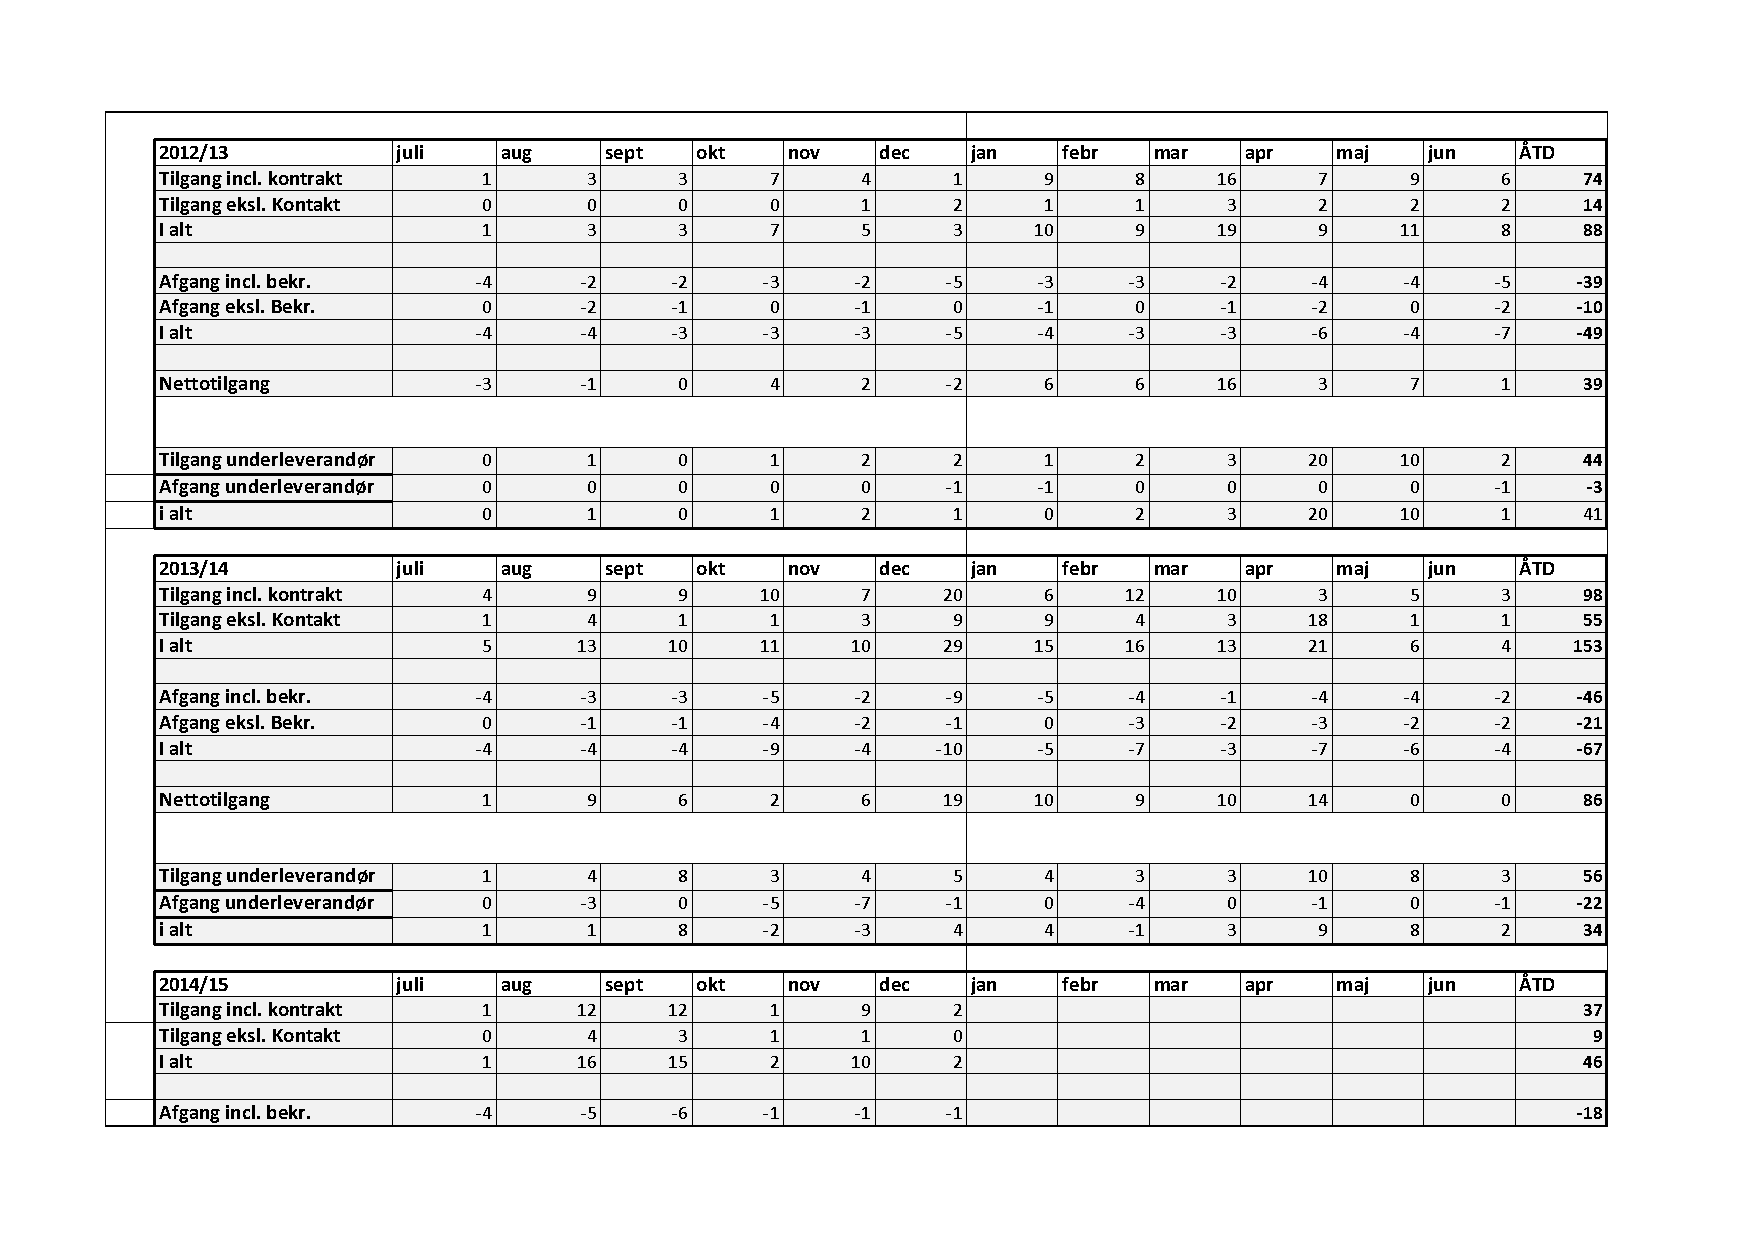
\includepdf[pages={-},scale=0.75,nup=1x2,pagecommand=\chapter{Recruitment data}]{appendix/recruitment_data.pdf}
\label{app:recruitment_data}
\chapter{SWOT analysis}
\begin{figure}[!htp]
\noindent
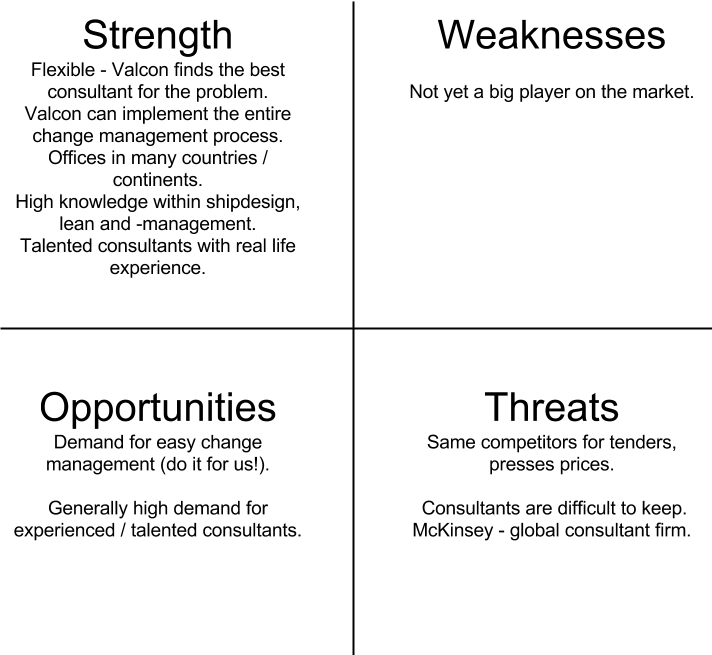
\includegraphics[scale=0.75]{appendix/SWOT.png}
\end{figure}
\chapter{Meetings}
\section{Initial meeting with Danni}
\label{app:danni_initiation}

\subsection{Summary}

The problem is defined as the recruitment process, the stress undergone during it, the amount of time it takes and how information is managed throughout it. Many different systems are used, and they must all receive data manually.
The process is not uniquely defined as it, in rare cases, must be done quickly, and thus the standardized procedure is not followed. This is mainly a problem for new OMT employees.

Valcon is already working on a new HR system to improve the way information is managed. Danni recommends a solution that automatises as much of the process as possible, to avoid human errors in insertion of new data.

Dannis goal for the project is to get a report that document that there is in fact a problem.

Valcons main business strategy is growth.
Their key values are that happiness and integrity is ensured for all employees. Furthermore, their consultants should be disturbed as little as possible.

\subsection{Minutes by Jonas Kastberg}
Introduktion:

Der bliver introduceret af de forskellige parter.
Danni er en gamer type
Vase er far
Jonas er der bare
Martin er også gamer
Merrild er også gamer
Michael arbejder her

Præsentation af vores projekt:
Vi skal lave en etnografisk undersøgelse
	- Det er spacy
Vi har brug for 2 møder senere på året
	- Det er intet problem
Der afleveres rapport d. 17 december
Der skal laves en underskrift



Danni: Hvor mange timer skal der bruges herude
Os: Det ved vi ikke
Jakob: evt. en 3 dage herude
Danni: Lisbeth kan være rigtig svær at få tid hos
Danni: Så længe i finder interessenterne kan jeg godt "spearheade"


Introduktion af Valcon:
Danni startede for 5 år siden
Eksplosiv vækst lige siden

IT og accounting vokser ikke meget iforhold til alt andet.
Dette besværliggører hyring af nye medarbejdere til Valcon og OMT
Lisbeth har ingen tid
Det er en meget konservativ kultur i firmaet
Problemet: Hvordan forbedrer man problemet uden at støde nogen i den kultur der allerede er.
Der er allerede en proces, men hvor automatiseres den.

Problemet: Processen skal identificeres, automatiseres og effektiviseres.

Efaring: Kultur og Proces hænger sammen

Afklaring af MUST:
MUST forklares, hver enkelt fase introduceres.
Ingen afklaring af Steering Comittee


Vores forståelse af problemet:
Der er en medarbejder der ansættes, og det kan tage lang tid.
	- Det er mere kompliceret at ansætte en medarbejde end som så.
	- Problemet ligger i hvordan arbejdet kan påbegyndes inden hyringsprocessen er færdigt processed
	- Lisbeth er bottleneck, da hun er den eneste der kan udføre processen
	- Der kan også være flere interressenter, Jytte og Niels hos OMT.
	- Problemet hersker hovedsageligt hos OMT.

Hvem er stakeholders
	- Danni (enighed)
	- Accoutning (Uenighed, foruden lisbeth)
	- Løn er som regel en bottleneck i firmaer

HR-afdelingen
	- Der er to HR medarbejdere, Bjarke og Hanne
	- Der et to medarbejder typer: Stationære og mobile

Nuværende løsning på problemet:
	- Igang med er HR system der kan bygges oven på det nuværende IT problem
	- Deres ERP (fakturering system) er 4 versioner gammelt (der benyttes Maconomy)
	- Evt. problem, streamlining af ERP Systemet. (java skal holdes på samme version for individuelle pc'er, da det ellers ikke understøtter maconomy)

Hvordan ser Danni processen:
	- Valcon melder ind til Lisbeth med en masse personlige oplysninger for ny medarbejder
	- Lisbeth putter det ind i systemet. (QHR, Lotus Notes egen udviklet system)
	- Andre grupper kan tjekke QHR for nye medlemmer.
		- Sekretariatet kigger derinde for at sende blomster og andre bløde ting (Vase likes)
		- IT tjekker og opretter brugeren i AD.
		- IT sender pc og andet til den nye bruger.
	- AD opretter brugeren på knowledge portalen.
	- AD Opretter brugeren på Lync
	- AD opretter mailgrupper til brugeren.
	- AD sætter brugeren i en sikkerhedsgruppe
	- IT opretter en mailbox til brugeren.

Eventuel løsning:
	- Automatiseret løsning for at Lisbeth kan godkende og så ryger det bare ind i QHR
	- QHR skal selv informere om at der en ny medarbejder.


Pipeline for at analysere arbejdspladsen:
	- Vi kan godt komme herud.
	- For kontakt med specialpersoner, kontakt med Danni for authorisation
	- Pipeline:
		- Skriv til Danni med hvem vi vil snakke med og om hvad
		- Danni skriver videre til personen og godkender os.
		- Vi skriver personligt til personen og aftaler tid og sted.

Motivationsfaktoren:
	- Vores sucess (ikke godt)
	- Hvis firmaet kan modtage en rapport der kan give en overbevisende forklaring om at der er et problem, og at det kan løses.


Firmastruktur:
	- Fire medarbejderværdier
		- Integritet
		- Glæde
		- Performance
		- Kompetence
	- Meget flad hierakistruktur


Business Strategy / IT Stategy:
	- Business Strategy = vækst
	- 

\subsection{Minutes by Michael Madsen}
Introduktioner:
Hyggelig stemning, hurtig introduktion af alle.
Vase bryder igennem. Vi skal lave en ethografisk undersøgelse. Det ved Danni ikke hvad er, så det forklares vagt.
Hurtig gennemgang af, hvornår vi holder møder.

Større forklaring af etnografi, og hvad vi skal med at observere.

Lisbeth bliver svær at nå på tid, Danni vil gerne 'spearheade' hvis vi selv identificerer dem, vi skal snakke med.

Danni introducerer sig selv kort, derefter Valcon. 340/350 mand. Fra 120 til 350 på 5 år, eksplosiv vækst.

Først var det Valcon Danmark, så Sverige, Norge, Indien, og så OMT da Maersk gav slip på OSS
Med sådan en stor vækst, hvordan skal IT og Acc så håndtere de nye, når nu de departments ikke er vokset så meget.

Problem: medarbejderne bliver ansat fra den ene dag til den anden, fordelen med intern IT er at det kan gå stærkt når der er brug for det.


Lisbeth er halvt HR halvt accounting, sidder med banker. Når det skal gå stærkt går folk udenom Lisbeth og presser på IT. Hvordan får vi en samlet pipeline uden at træde på nogen tæer. Dem der beder om at få ansat, Lisbeth som skal indtaste, IT som skal lave udstyr og have information.

Mulig udvidelse: hvordan kan vi automatisere fratrædelse?

Vi snakker om hvorfor det skal være IT. Formålet med faget, Danni er enig i at faget er en god idé.
Vi forklarer hvad MUST er:
initiation phase, vi skal forstå hinanden, blive enige om problemet. osv.

Vi forklarer hvad vi har forstået. 
Danni forklarer - man finder ofte rigtig sent ud af at en ny medarbejder skal ansættes. IT kan lave en bruger hurtigt så folk kan i gang, Lisbeths opgave i HR kan godt vente et par dage, men det er dumt fordi lønninger og hvem betaler hvor.
Vi kommer frem til at problemet er, at flere ting skal laves samtidig.

Politik: vi bør ikke nævne overfor Lisbeth at der måske kunne være flere som kunne udføre hendes arbejde.

Problemet er oftest OMT fordi der går det rigtig rigtig stærkt.


Stakeholders: Danni, Lisbeth, IT afdelingen, OMT. Ikke andre end Lisbeth fra accounting.


Der går lidt snak i den omkring at der altid er én der sørger for lønninger.


"Er der en HR afdeling?" Nej, der er Lisbeth. To HR medarbejdere, Bjarke og Hanne, BJR og HNO, måske kunne vi snakke med dem.


Det er fragmenteret fordi OMT har deres egne folk til sine ting, Valcon til sine egne ting. To forskellige forretninger. Valcon er management consultants, er mobile og rundt omkring. Omt er faste, med dock, 2 skærme, tung PC, tegner skibe.


I gang med at finde en løsning: Valcon kigger på et HR system for at se hvor meget af processen der kunne ordnes i et nyt samlet system. 
ERP systemet (fakturering osv). Vores Maconomy er 4 versioner gamle, vi må ikke opgradere java fordi i vores kontrakt må vi ikke køre ny Java, for vi skal betale hvis vi skal opgradere Maconomy, og noget customisering vil gå i stykker.


Danni har ikke været i så mange møder omkring det nye HR. Men Danni siger at vi vil have moduler, ikke ting der går i stykker ved hver update.
Hyggesnak om ERP systemer og at de er fucked up.


Den aftalte process: Lisbeth skal have fødselsdag, adresse, email, stamdata. Når Lisbeth ahr det, putter hun det ind i QHR. Det er Valcon/OMT som skriver det her til Lisbeth. Det er den som ansætter, men det er ligemeget.
Danni foreslår at lave en formular til Lisbeth, så det bliver standardiseret.
Lisbeth lægger ind i QHR ( egenudviklet database i Lotus Notes ). Flere modtagere herfra
IT kan læse det, sekretærerne kan læse det og sende blomster. Der er *måske* andre som bruger det. Det kan være accounting kigger derinde, who knows.
IT laver AD bruger. Der bliver automatisk trukket fra AD til Knowledge Portalen. IT opretter mailbox på Exchange serveren. Fra AD bliver folk også automatisk Lync enabled, i PC to PC version. De bliver automatisk lagt i mailgrupper og sikkerhedsgrupper.
Comment fra Rasmus - Vi er the 'how'. McKenzie som konkurrent?
Vi skal finde møde-datoer og sende til Danni. Vi skal skrive project charter (kontrakt) og sende til danni inden tirsdag.
Note til Danni. Jytte eller Niels eller en anden fra OMT for at høre om deres ansættelsesprocess.

\section{Meeting with Danni after in-line phase}
\label{app:danni_inline}
\subsection{Summary}
During the interview, we show Danni the progress we've made and what we've come up with. 
He mentions that the size of Valcon is both a boon and a bane and explains Valcon's situation in the market and how they stay in the competition despite not being the biggest firm. 
Valcon are good at being with a project from initial to implementation and the projects they put out offers on don't see a lot of competition, so they generally know who they're competing with. 
OMT's choice of working with subcontractors is a conscious decision as it's part of a strategy for the company.

\subsection{Interview notes}
Michael: Hvad er vores forståelse af Valcon og hvordan vores forståelse af processen ser ud
Vi viser vores canvas frem og forklarer hvad det går ud på og hvad vi har skrevet
Danny foreslår at vi skriver ‘the how company’ på, det ville Poul være glad for

Michael: Vi har ikke fundet noget specifikt segment for Valcon\\
Danny: Der er også medico og rejseselskaber/flyselskaber. Det man kan sige er at public sector ihvertfald ikke er den største, det er industry/medico hvis man ser bort fra skibsdesign. Han syntes vi skal specificere at det er i 'no particular order' eller rykke public sector nederst ihvertfald.

Michael: [Det her er de] channels [vi har kigget på]\\
Danny: Relationship building er også en ting, dem der arbejder her ude har en kæmpe kontakt bog på 3500 kontakter som de kan hive på.

Michael: Key activities + key resourcer\\
Danny: I kan inkludere 'experience in how to' under key resources

Michael: Value propositions\\
Merrild: De der Kurser Valcon holder, er det substant?
Danny: Nej, det meste af det er udfakturering. Sales skal måske stå i bunden, da deres absolut største key activity er projekter.

Michael: Cost structure + key partners\\
Danny: Vi driver os selv, ja. Practical costs har en subkategori der hedder 'husleje'. Det ser ihvertfald godt ud.

Michael: SWOT analyse\\
Danny: SWOT analysen burde nok være på engelsk\\
Danny: Strength: Stor viden indenfor skibsdesign, lean og management

Michael: Valcon er sandsynligvis ikke de største? Er det korrekt?\\
Danny: Størrelsen af valcon er både en styrke og en svaghed. Vi har opgaver hvor vi kommer ud hvor Mckensy har lavet rapporter og analyser og så kommer vi og faktisk implementerer det, fordi det kan Mckensy ikke finde ud af.

Michael: Det at OMT skal bruge udefrakommende arbejdskraft er måske en weakness?\\
Danny: Det er helt klart en del af en strategi, fordi så kan de hurtigt udskifte arbejdskraften uden at skulle tænke på kontrakter og andet\\
Danny: Vi vil i virkeligheden gerne have flere store projekter, så hvis vi er hos DSB vil vi hellere lave flere medium størrelse projekter i stedet for ét stort, fordi de forskellige projekter kan yderligere udmunde sig i flere projekter

Michael: Der er ikke mange ligesom valcon\\
Danny: Lige præcist, 'the how to company'\\
Danny: Mckensy har rigtig mange unge ansatte, hvorimod valcon har mindre unge men rigtigt mange i midter segmentet. Så vi har mange der kan finde ud af at implementere tingene fordi de allerede har været ude i feltet, hvorimod Mckensy har mange unge som kommer direkte fra uddannelser og derfor er gode til at skrive rapporter\\
Danny: Der er mange ude at byde, men der er ikke mange om de bud som Valcon byder på. Det betyder at det generelt altid er de samme som byder og derfor kender de hinandens priser, svagheder osv.\\
Danny: Mckensy er større og derfor har de mulighed for at være competitive på priser og deres yngre konsulenter er billigere end de meget kvalificerede konsulenter som Valcon har.\\
Danny: Vi er selvfølgelig interesseret i at holde i vores konsulenter. Det gennemsnit som folk er i Valcon er generelt op til 5 år som ligesom grænsen for hvor det bliver svært at holde på konsulenterne. Mckensy har ikke noget imod bare at skifte deres klientel ud efter nogen år, de tager bare nye fra universiteterne

Michael: Forståelse af ansættelses processen, forklaring af vores flow chart, forklaring af vores interviews og hvad vi har fundet ud af\\
Danny: Kunne det være gavnligt hvis man med en graf at vise hvor mange reelle ansættelser det handler om?\\
Os: Ja, det ville være fedt med konkrete tal

Michael: Valcon kommer til at ansætte flere, det mener Jytte ikke at OMT kommer til. OMT kommer til at give slip på en større mængde mennesker, men ansætter dem senere igen\\
Danny: Hvad er next step for jer?

Merrild: Vi skal have skrevet alt det her ned og så skal vi have fundet faktiske løsninger. Derfor ville det hjælpe meget med konkrete tal\\
Danny: Det kan vi godt finde ud af, I kan bare spørge Lisbeth om det. Grafer og reelle tal mangler I generelt, det ville gøre det rigtig godt hvis I kunne få noget direkte substans i det med konkrete tal.\\
Danny: Cirka halvdelen af pengene kommer fra OMT

Merrild: Udfakturerer I forskelligt baseret på hvilke konsulenter der bliver brugt?\\
Danny: Ja, det gør de. Der er forskel på hvilke konsulenter der bliver solgt af tid for, så det betyder at der er dyrere konsulenter og mindre dyre. En konsulent fakturer imellem 1500 og 2800 i timen. Det dækker så også over flere ting, praktiske expenses inkl pc, transport, telefon og så videre.



\chapter{Interviews}
\label{app:interviews}
Each of the following interviews are prefaced with a summary giving a notion of the key points retrieved.

The interviews are written in danish, and has not been edited since they were made, in order to avoid tampering.
For clarification in some cases, notes has been added, denoted with [ ].

\section{Generelt fra Michael}
WRITE IT

\section{Interview with Hanne 21/10/2014}
\begin{linenumbers*}
\subsection{Summary of Interview}
Hanne is partly responsible for all hires in Valcon. She manages job interviews, DISC profiles and cognitive tests (partially), as well as planning meetings and communication between Valcon and potential new hires. \newline
Currently, this process involves a lot of manual data entry in a private excel sheet. 
Most of Hannes process is outside of the scope of this assignment, however a few key points from the interview were important:
\begin{itemize}
	\item{The hiring process in Valcon is sometimes chaotic, with consultants that start on short notice, or with key information missing. It should be possible to make PC's for new hires anyway, as their time is very precious}
	\item{Hanne manually updates a lot of information in a private excel sheet. A lot of this information is shared with Lisbeth, and could be moved to a shared system. This would also reduce Valcons dependency on a few key persons.}
	\item{Sometimes, the reason Hanne does not have the needed information for Lisbeth is because the general attitude amongst some consultants is that it isn't urgent}
	\item Hanne is not an actual recruiter at Valcon, however she is a big part of the process.
\end{itemize}
Furthermore, it was mentioned that no further tasks should be given to the consultants.

\subsection{Interview Notes}
\label{app:hanne_interview}
Hannes process:
Som det er nu, er det rigtig håndholdt. Meget personafhængig. 

Der er forskellige veje ind. En ansøger kan kende en fra Valcon, sende CV til ham/hende, det ryger videre til job@valcon.dk som styres af Hanne.
Hun behandler alt - "tak for din ansøgning, vi kigger og vender tilbage til dig". Det er Hanne. Intet automatisk.
Hanne screener ansøgninger. Hvis de er tydeligt irrelevante, beslutter Hanne at sige nej tak direkte. Tvivlstilfælde sendes videre til Bjarke, som er recruitment manager, (han finder også folk fra linkedin og andre steder).
Hvis det måske kunne være interessant i en given afdeling, sendes CV'et videre til en chef for at høre hans mening. 

Hvis svaret er ja, så skrives der tilbage til ansøgeren "vi har kigget på dine papirer, vi vil gerne se dig til vores rekrutteringsproces til trin 1: et interview" Der møder man Bjarke, nogen gange også nogen fra forretningsområdet.
Her kigges der på personlighed. Det varer en times tid.
Hvis det er nej tak, så ringes der "nej tak". Hvis personen har været på Valcon, bliver det altid personlig henvendelse.

Hvis kandidaten er velegnet: kognitiv test og DISC test. Send link til DISC profil, invitér ansøgeren til at komme til test + tilbagemelding.
En uge fra link til møde. Det er altid Bjarke der tager mødet. Hanne laver den kognitive test. Bjarke er certificeret i DISC og kognitive test.

Der kan snakkes med Camilla Huus, hvis det er en spændende person men vi ikke lige ved hvor personen vil passe. 

Hvis det bliver go, så skal vi have et møde med den ansvarlige i det forretningsområde som det skal være i. En times tid, holdes af Hanne.
Hvis det går godt, sidste del. En casepræsentation, hvor Hanne sender en case til ansøgeren, og ansøgeren får en uge til at forberede casen.

Herefter et møde, hvor Camilla eller COO altid deltager, plus den ansvarlige for forretningsområdet, same Hanne eller Bjarke. Det er en form for rollespil.
Ansøger præsenterer i cirka 1,5 time. 
Herefter voterer de om hvordan det gik. 50\% går igennem, cirka. Casen er meget afgørende.

Efter det her er der et møde om løn, ansættelsesvilkår, salgsmål, bonusmål. Det skrives ned på et stykke papir som Lisbeth får. Hun laver kontrakt. Så er Hanne done.

Hvis afslag ringer en chef til ansøgeren og giver feedback på hvorfor det ikke gik. Det går rigtig godt. Hanne får søde mails fra folk som får nej tak.


Processen er flydende og tilfældig, den med information til Lisbeth. 
Mange forskellige variationer:

I den ene grøft, en konsulent kommer ned til Danni og siger "nu kommer Thorkild jo så i morgen. Der skal være en PC klar". Danni siger "hvem er han?" "ham har vi lige talt med så han starter om et par dage".
Samtidigt ind til Lisbeth "Ham her skal have en kontrakt lige nu, her er hans info. Lav en kontrakt."

I den anden grøft, efter kommandovejen. Efter voteringen sendes der en mail til Lisbeth fra Hanne. Hun [Hanne] skriver at der skal laves en standardkontrakt til XX. I mellemtiden findes salgsmål og bonusmål. Tilføjes i endelig udgave af kontrakten.
Der er standardkontrakt og så den endelige. 
Standard: efter case præsentationen, når vi ved han skal ansættes [en template, med basis information]
Endelig: [Når vi har fastsat løn og salgsmål]

[I] den gode process lægger Hanne CV over i Notes [QHR], Lisbeth får at vide hvad hun skal gøre, her er salgsmålet osv. Send en PDf til ansøger, så han kan se den før den printes og sendes.

Hvis Hanne skulle give et bud på det perfekte system:
Noget af det her håndholdte, skal ske mere automatiseret. men der skal stadig være mennesker til at udløse handlingen, of course. 
Efter casepræsentation, en besked til Hanne om at "vi vil ansætte sådan og sådan", Hanne ved at processen er afsluttet og kan registrere i sit excel ark, hun kan sende det videre til Lisbeth.

Somme tider svæver det lidt hos Hanne hvis ikke hun ved om de er endt med at blive ansat eller ej.

Der lægges et stamblad med bankkonto nummer ved kontrakten. Alt muligt skal udfyldes. Det er ikke alle der udfylder det. Og ofte haster det lidt eller meget. Ofte ringer man. Så det er [Rest of the sentence was lost]




Spørgsmål:
Hvor sure vil folk blive hvis IT siger nej til PC om 2 dage
Svar:
Sådan en som Thorkild [Et eksempel vi fik på en ansættelse der skulle gå alt for hurtigt], han kom ud af det blå. Intet CV, intet interview, han skulle bare ansættes på grund af netværket. Vi ved at han er den helt rigtige til opgaven. Bum, han skal på et projekt lige nu.
Det er her vi adskiller os fra de meget firkantede hvor ting ikke kan lade sig gøre. 
Vi gør det fordi det er vigtigt for virksomheden, det er nødvendigt. Når jobbet er der, skal det bemandes.
Kunderne skal have konsulenter ud med det samme.

Hanne har jo også masser af jobsamtaler klokken 7 om aftenen. Vi må være fleksible.


Brainstorm: IT har altid klargjort 3 PC'er som mangler at få "det sidste". Det belaster selvfølgelig vores cashflow, likviditet, IT.
Altså at lave en buffer så der er PC'er mere klar. 


Der er problem med dem som sender info for sent. Det er et problem alle steder. Hvordan får vi fat i dem.


Organisationen ønsker ikke at alle må tilgå systemet. Der må ikke lægges flere opgaver ud til konsulenterne. (det går imod Lisbeths drøm om indtastning af kurser osv.)
I den ideelle verden kunne en chef lave en rekvisition og bede om medarbejder, og alle var aktive i systemet. Men det kommer ikke til at ske, for han  [chefen] har for travlt.
Cheferne har for travlt. Det er en beslutning Rasmus har taget. "Det er godt at vide at det findes; det kommer ikke til at ske.". I hvert fald ikke mens Hanne er her.

Spørgsmål:
Hvorfor findes der ikke en standardiseret mail?
Svar:
\linelabel{hanne_standardised} Den vil ikke blive brugt. Af samme årsag som tidligere.  [at processen skal kunne være flydende]
Vi er i Valcon meget tilbageholdne med at bruge standarder.
Nogen ville være med på den, men der er flere som så sender en sms i stedet, for at komme uden om.

Organisationen er ikke klar til flere systemer. Det er nogen som vil være med på det, men der er for mange som ikke er.


Det som mindkey ville kunne:
Det kan afhjælpe et hav af de opdateringer Hanne laver på sit excel ark. 


Målet for Hanne:
I stedet for at skrive en mail til job@valcon.dk så henter man et skema og udfylder, som automatisk siger "tak for ansøgningen" med rigtig udfyldt data i mailen.
Hanne skal altid kunne give status på pipe, på disc, på case. Alle de her ting opdaterer hun selv. Hvis det kunne ske automatisk jo mere hjælp får jeg.
Men det må aldrig ske uden at Hanne har givet lov.
Bliver sommetider lidt overvældet over at skulle booke i 2 kalendre ved invitation til Disc, skal sende et link, bestille et nyt link, mange småting. 

Det kører godt for Bjarke - han har kun de funktioner han skal. men han blev også ansat til det; recruitment manager. Men Hanne skal rigtig rigtig mange ting.


Det kunne også være en del af løsningen at kommunikere bedre om, hvad der er et stort pres på IT afdelingen. Så folk har lyst til at gøre ting i god tid.
\end{linenumbers*}
\section{Interview with Jytte 4/11/2014}
\begin{linenumbers*}
\label{app:jytte}
\subsection{Summary}
Jytte believes it would be beneficial to have a standard form for recruiters in OMT to fill out.
The standard form should contain fields for all the information required by accounting and IT.
Some information should not be on the form, e.g. salary information, because it should be shared with as few as possible.
She doesn't believe that the hiring process will happen more often, because it has never been a strategy for OMT to grow as much as they have.
On the other hand they will continue to let go of and rehire subcontractors.

Jytte also believes that it would be a good idea to have a supply of PCs and mobile phones in OMT, as well as having an IT employee at OMT every day, instead of the ~3 days every week that is currently there, to improve response time.

\subsection{Transcript}
Michael:
Lidt om det vi laver. Vi har et stort fag, BFOP.

Jytte:
Hvad læser I?

Michael:
SWU[Software udvikling], men ITU vil gerne have nogle udviklere
der kan andet end kode.
[Forklarer om hvad BFOP og projektet går ud på]
Danni foreslog ansættelsen processen. 
[Forklarer de dele af processen som vi kender til]
Vores opgave er at lave buzzcase. Vi har snakket med Peter,
Lisbeth og Hanne. Vi vil gerne høre hvad processen er i OMT?
Vi har hørt det er dig.

Jytte:
Det er sandhed med gran salt. Alt hvad der er
Underleverandører, skæve, midt i måneden, ikke standard.
Hvis ikke man har en standard platform, så i hvert fald
en standard template. 
Hvordan bestiller man ny medarb. En template der dækker hovedparten.
\linelabel{jytte_standardised}
Vi deler ikke ansættelsesforhold, løn bonusser etc. med IT.
Nogle ting skal deles med alle. De ting kan lige så godt være
standardformularer.
Vi er ISO certifiseret. Der ligger mange standardformularer,
den kunne ligge samme sted.

Michael:
Som fastansættelser, hvordan er processen i OMT.

Jytte:
Lige som Valcon, hvis ikke personen kendes så godt så første interview. 
Synes man match så tests. Bruger ekstern HR konsulent til at klare tests.
Det der ikke kører per automatik. Ligge DISC profiler ind på CV. 
Har for nyligt formidlet til Hanne om hun ikke kunne ligge dem ud.

Michael:
Så info til Lisbeth kommer ud efter sidste samtale?

Jytte:
Efter tests så ny samtale. Hvis ansat så bestil kontrakt hos Lisbeth.
Hun får al data fra mig.
Så kommer den i papir fra Valcon. Nogle gange som PDF.
Det behøver ikke standardiseres. 
Så sender vi svar kuverter med. Laver en aftale med ansatte
om at de skal sende til Lisbeth.
Men når de har sendt så bedes de sende en mail til mig. 
Når Lisbeth modtager kuvert, så sender hun også mail til Jytte.
Det sker at kuvert ikke når frem til tiden.
Det skal være fast procedure at Lisbeth bekræfter at hun har modtaget kuvert.

Michael:
Hvor meget er du med når det er eksterne kandidater?

Jytte:
Det varierer. Nogle gange så ringer fo
[faglederen til mig of fortæller at der er en på vej. 
Andre gange så får jeg ikke noget af vide.]

Michael:
Hvem bestiller?

Jytte:
\linelabel{jytte_stamdata}
Faglederen. Vi har nogle gange pladsproblemer i OMT.
Jeg mangler også at få information omkring nye underlevenrandører fra faglederen. 
Der er skal være en standard formular som skal udfyldes med stamdata
+ hvilken PC der skal bruges. 
Jeg tror I bruger 3 kategorier(af pc)

Michael:
Jo, vi har 3 men det er også ved at blive lavet om afhængigt af lager.
Det her med at sende info til Lisbeth,
bestille kontrakt osv er det noget du bruger meget tid på?

Jytte:
Nej. Har efterhånden bestilt så mange. God kommunikation.

Michael:
Kommer denne her process til at ske oftere?

Jytte:
Nej, det tror jeg simpelthen ikke på. Men det har jeg jo sagt før.
Det har aldrig været vores strategi.
Så skal vi til at vokse her(Hørsholm), men det har vist sig svært.

Michael:
Oplever du nogle gange det ikke går stærkt nok?

Jytte:
Ja, men det er jo svært. Der er altid nogen der ikke synes det går stærkt nok.
\linelabel{jytte_buffer}
Hvis vi skal forbedre noget, så skal vi have et standard lager med PC og telefon.
Problem at Allan ikke altid er i Odense.
Vi har jo også snakket med Rasmus og Danni om det, ved godt at der er lidt presset i IT.
Når der kommer en ansat mere i IT så kommer Allan mere til Odense.

Michael:
Vi har snakket om lager af færdige PC’ere. Så det kan gå hurtigere nogle gange.

Jytte:
Ja, nu er der jo det eksempel når der skulle gå til at ...

Michael:
Nyt HR system?

Jytte:
Ikke hørt noget, OMT ikke en del af det nye HR system.
Enten skal OMT bare have det, eller også skal de ikke være en del af det.

Michael:
Det der er snak om for at lette komm mellem Hanne og Lisbeth,
er et program der ville være. Smart?

Jytte:
Det løser ikke vores problem, for underlevenrandører ikke i det system.
Hvis man skal bruge sådan et system så bliver jeg flaskehals.
Jeg skal ikke være HR ikke mit job, vi har bare ikke nogen HR. 

Michael:
Hvad er dit job?

Jytte:
Ansvarlig for projektservices her, OMT og Kina.
Det er ikke mit job at sørge for at der er borde til folk.
Har ikke lyst til at være flaskehals for bestilling af PC’ere til nye underleverandører. 

Michael:
Der er ikke nogen ...

Jytte:
Pludselig en hel masse. Jeg kan sagtens sige at alle skal udfylde den her blanket,
men hvis sekretær skal indtaste det ikke godt. Jo færre der ved noget om løn jo bedre.

Michael:
Mest underleverandører der er mega travle?

Jytte:
Ja, der er undtagelser med fastansættelser, men det er ikke ofte.
For mange kokke om maden, 
Hvis vi skal bruge QHR(nye HR system) så skal vi ind over.
Det skal ikke være lige som portalen. Vi bruger ikke portalen.
 
Michael:
Bruger i filesync?

Jytte:
Meget meget lidt. Vi tjekker ikke meget ud, og må ikke.
Vi får ikke lært at bruge dem.
75\% af vores medarbejdere rejser ikke. De møder ind på kontoret hver dag og arbejder.
Hvis der er et HR system der kan bruges til gavn for Lisbeth og IT
så vil jeg gerne være med til en dialog om det. 
Men vi gider ikke det bølv der er med 

Michael:
Recap

Jytte:
Tving underlevenrandører til at svare det på alting.
Vi udlevere ikke tlf til underlev.
Nogle gange får de ikke tlf. med fra arbejdsgiver, så skal de have fra os(vikar).

Michael:
Mere IT i Odense en god ting?

Jytte:
Business objects rapport - det er derfor underleverandører skal i korrekt department

Merrild:
Hvor længe varer en ansættelse?

Jytte:
3 måneder, 2 år, det varierer. De må kun arbejde på vores platform, 
vores servere, vores PC, fordi det er et lukket projekt.
Det er derfor alle skal have en PC. Ingen clouds involveret.
Det er i høj grad på grund af det Canadiske projekt
at vi har brug for så mange underleverandører der skal have PC’er. 
På trods af det går vi meget efter lignende projekter.
Der er rigtig rigtig mange penge i det i forhold til kommercielle skibe.
Så det kommer til at ske igen.
Grunden til at OMT ikke vokser mere, er fordi der ikke findes flere i Danmark
med den viden om skibsbyggeri. 
Jyttes bud er at der er cirka 55 underleverandører nu.
Vi forventer at hvis der kommer et nyt projekt bliver der ringet til dem igen,
og så skal de have PC igen.
Måske lade være med at slette eksterne accounts,
lukke dem op igen når de kommer tilbage.

Det bliver et issue at hardware bliver forældet,
når alle sendes hjem når projektet er færdigt.

Konkurrenter:
Rosteen Knudsen, Knud E Hansen, HC consult, Shipcon. Principia North i Svendborg. 
Logamatik og Wilhelmsen kommer der el og automatik kompetence fra.
Vi bruger nogen fra : Process engineering. De laver rør.

KEH vil hellere lave roskibe og færger end de vil lave containerskibe,
og OMT vil ikke lave færger. Så det er ikke fordi der er konkurrence mellem
firmaerne. 
Konkurrence om de gode medarbejdere, men ikke andet end det.

Kategori vi ikke har snakket om: timelønnede.
De har ikke noget garanteret timetal, men de skal også have en PC.
De får normalt kun en PC. Er det en som bare kommer ind til f.eks.
et værfts-optimerings-projekt som varer 3 måneder,
så skal de også have PC i bare 3 måneder.

Underleverandører får ikke løn fra os. Vi får en faktura fra dem. 
Med timelønnede håndterer vi betaling af dem, dvs Lisbeth.

Eksterne får et X foran deres initialer. Jeg ville hedde XMM, f.eks.
Når der søges på X kommer alle eksterne frem, og en gut der hedder Alex.
Måske et issue.

De bruger business objects til at se hvor mange timer
de forskellige medarbejdere er belastet hver måned.
Så det er godt at kunne sortere efter X’er.
\end{linenumbers*}
\section{Interview with Lisbeth 21/10/2014}
\label{app:lisbeth}
\begin{linenumbers*}
\subsection{Summary}
Lisbeth is an extremely important part of the hiring process. She is solely responsible for managing contracts for employees, and keeps a lot of data in private, local files. 
For Lisbeth, communication starts when either Hanne (Valcon recruitment), Jytte (OMT recruitment) or someone external (from departments outside of Denmark), writes an email with information on a new hire.
She manages the creation of contracts, maconomy accounts and salary systems.

From the interview, we found these key points:
\begin{itemize}
	\item{The old system was better for Lisbeth.}
		In the good old days, Valcon used Lotus Notes for everything. Lisbeth could automatically send mails from new employee data, and a lot of automisation was in place. During the years, more and more key functionality was removed from the Notes platform (invoicing was moved to Maconomy, mail was moved to Outlook, account management moved to Microsoft Active Directory). This slowly removed all the special functionality of Notes as an integrated solution.
	\item{Lisbeth has too much important information in her head.}
		 It is part of her job to have an overview of the pipeline of incoming and outgoing employees, and most of that is currently kept either in private excel sheets, or her head.
		 This is not good for a business.
	\item During the process, Lisbeth inputs a large amount of data manually
	\item Lisbeth supports the idea of a more automised process, and believes that IT should not accept hires directly going to them, as they should always go through Lisbeth.
	\item Lisbeth believes that a good solution would be to have a huge end-all system that everyone helps keeping up to date, with information about most things.
	\item{The hiring process for Lisbeth is not time consuming in itself.}  
		She uses 10-15 minutes per employee, best case. The problem arises when information is missing in mails from recruiters, as well as the inherent problems with copy-pasting information several times.
\end{itemize}


\subsection{Interview notes}

Interview med Lisbeth
Introduktioner
9:30

[M:] Hvad sker der når en ny skal ansættes i Valcon?

[L: Jeg er] ansat til at lave løn og kontrakter
Når Hanne og Bjarke har fundet en medarbejder de vil ansætte skriver de til L[isbeth] med navn adresse og CV, hvornår han skal starte og hvilken afdeling.
Hvis hun er heldgi (H eller B [Valcon recruiters]) skriver [de] det selv ind i QHR. Så har L[isbeth] basic info. Notes understøtter ikke den organisation de har i dag, så [der] kan ikke tilknytte afdelinger/ løn / managers på "60\%" [af de nyansatte]. Når jeg får den lagt ind laver jeg en kontrakt. 
\linelabel{lisbeth_kontrakt}
Jeg skriver [sender] denne til kandidaten som underskriver kontrakten.
Så skriver jeg en mail til rekruttør at kontrakten er underskrevet. Går ind i Notes og ændrer kontrakten fra rekr.[utterings] process til ansat. Klikker på en knap så den laver skema til IT. Nogen gange har de [Hanne og Bjarne] ikke lagt stamdata ind, så skal jeg selv hente det.
\linelabel{lisbeth_IT}
Skriver nu selv en mail til IT om at de er kommet.
[Når de kommer fra OMT, skriver] Jytte fra OMT, [nogen] skal ansættes, navn, data, CPR, afdeling. Det er ikke altid jeg får lønne[n] at vide. [Jytte] Glemmer [nogen gange] start-dato [hvornår de starter med at arbejde]. Løs mail. Nogen gange er der kun 80\% af data.
Mail dialog om kontrakten [mellem Lisbeth og ?].
[Tanke- Meget snak om good old days (QHR ordnede meget selv, gav selv grundløn, alle indtastede derinde).]
\linelabel{lisbeth_vende_tilbage}
Nu skal jeg vende tilbage til rekruttør 99\% af gangene [og bede om mere data].
[I] 2009 var der i gang med en ny database, men den blwv stalled. Så kommer Outlook, og så dør Notes. Afdelinger, ledere etc. bliver ikke ajourført i Notes, så når jeg sender en mail [til ?] skriver jeg i headline på mailen ANSAT I ... MED CHEF ...
Man kunne søge på ting i QHR, hvilket man ikke kan længere. Se hvem der var under ansættelse, se hvem der var ansat. I gamle dage kunne man se hvad der lå i rekrutteringsdatabasen, og det kan man ikke i dag.

M[ichael siger] - Sværere at få et overblik?

\linelabel{lisbeth_ark}
L[isbeth svarer] - Ja
Hanne styrer det i et regneark, Lisbeth har også kontrakterne i regneark. Styrer det på en anden måde i dag. Hvis vi ikke er her er "fanden løs i laksegade". Der er ikke nogen udefrakommende som kan lave noget [i rekrutteringsprocessen]. Overleveringen til en ny medarbejder er stor. Folk der har været her længe og kender processerne.

[M:] Bliver problemet større?

[L:] Ja, organisationen bliver større / ændrer sig, og mindre og mindre passer i databasen. Der mangler information om OMT i systemerne. 
(Andet problem:)
Jeg kan ikke vide om en kandidat bliver til en ansættelse, så hvis han pludselig springer fra skal alt slettes. [Det] sker af og til.

[M:] - Skal det gå hurtigere end tidligere? Tænker på OMT, 4 dage...

[L:] Ja... Fra midt juli til nu kun 1 konsulent, 8 fra starten af November. Mette har ikke adgang til QHR (sekretær i OMT), ringer og spørger om hvem der starter i Nov, men det kan man ikke vide før måneden er forbi. \linelabel{lisbeth_overblik} Alle tror jeg har overblikket. Men glemmer jeg noget er det væk. Det står og hviler på mig.

[M:] Sker det at IT får noget at vide først?

[L:] Ja... En gang imellem tror jeg. Det kunne ske mere tidligere, men nu har jeg opdraget Indien [hvor problemet var størst]. Vi skal også styre alle underleverandørerne, de skal starte dagen efter, de er blevet lidt bedre, men det er stadig slemt. \linelabel{lisbeth_standardiseret_proces} IT skal afvise dem og sende dem til mig. De må ikke have adgang til vore systemer, men de skal have en mail fra os og nogle initialer, så vi kan lægge dem på projekter og timeregistrere. Derfor skal de oprettes i Maconomy, de kan få adgang til vore systemer gennem en App, hvilket de godt må. [Om initialerne:] IT tildeler initialerne, for de har skøre hjerner. Det fungerer fint --- vi snakker lidt om om det skal være anderledes, vi kan få systemer som kan understøttes.

[M:] Det nye HR-system?

[L:] Mindkey har vi snakket med, intuitivt og virker godt. De skal forstå vores case. [De skal ikke vende tilbage med et] hov der vra lige noget. Til at gå til og prisen er ikke vanvittig. Så må vi se. Der er jo det at man kigger på økon. fee hvert år, hvor mange brugere, alle skal ikke have adgang, forhandle en anden pris for mindre adgang. Jytte/Hanne/sudo/balla/Pelle/Mat [sudo og balla er indiske ansatte, Pelle og Mat ved jeg ikke hvem er] skal have fuld adgang, og kan ligge ind i systemet. Jo kortere vej jo rigtigere oplysninger, [for eksempel] Jakob med K eller C. De skal så køre hele processen i systemet, så de får meget hjælp, og hvis der sker nogen noget så ligger de der.

[M:] Det nye skal være ligesom QHR var engang?

[L:] Ja. Samspillet skal op og køre igen. I mange andre virksomheder rekvirerer de [sådan her:] "så rejser der en, så kommer der en ny". Vi har ikke ledige stillinger. Ikke på konsulentsiden, måske på backoffice. Hvis den rigtige ikke er der ansætter vi ikke nogen. På den måde er vi anderledes ([det er et] problem i forhold til det nye system). Løn er salgsmål og faktureringsmål. Der er ikke lønklasser, det er individuelt. Erfaringsmæssigt forskellig løn, og det skal systemet understøtte. Det skal ligesom skræddersyes til os. Vi har ikke holdt opfølgningsmøde, men Mindkey var det bedste af 3-4, der er masser af HR-systemer. Ofte er der kun rekruttering eller noget andet.

[M:] Valcons udfordring er at deres organisation er så anderledes?

[L:] \linelabel{lisbeth_HR} Ja, det nye system er Microsoft baseret, så de skulle kunne snakke sammen. [Her snakker hun om problemet med at systemerne ikke kan snakke sammen. Specifikt Maconomy og Lotus Notes.]
Jeg har også et lønsystem.
\linelabel{lisbeth_manuelle_indtastninger}
[Beskriv hele processen:] Jytte skriver mig en mail, jeg tager oplysningerne og lægger dem i QHR, så taster jeg det ind i Maconomy, og til sidst i lønsystemet. 4 manuelle indtastninger. Man kunne i hvert fald få et step væk. Det danske lønsystem (bluegarden), norsk revisor og svensk system. Revisor i Canada, engelske lønninger hos Dorthe. Indien og Kina klarer sig selv. Alle skal igennem mig, for alle skal have adgang til medarbejderne i Maconomy.

[M:] Hvor meget tid bruger du på ansættelser?

[L:] Det fylder meget. Det er manuelt det hele.

[M:] Hvad med hvis det hele er der i QHR? 

\linelabel{lisbeth_time_spent}
[L:] 15 minutter for kontrakten. Maconomy 5 minutter ca. Samme i lønsystemet. Problemet er når der skal snakkes sammen meget. Nogen gange sidder man og roder lidt[, finder på småting for at få det til at hænge sammen]. Finpudsning er der ikke plads til. Hvis man havde valgt Maconomy til medarbejderstyring, kunne det være nemmere, men det var dårligt så det blev valgt fra. Den er død[, Maconomy skal ikke styre medarbejdere]. Der skal vedligeholdes på medarbejdere. Mindkey skulle også kunne udstyr. Vi ser på det hele. Ansættelse, vedligeholdelse, afsked. Hvorfor siger medarbejdere op, det skal også kunne blive i systemet. Hvorfor smider vi selv folk ud? [Det skal også være i systemet.]

[M:] Skal du give grønt lys?

[L:] Ja, når jeg trykker ansat får IT det at vide. Jeg er ikke interessert i Hannes database, og de skal ikke kunne se hvad der sker i OMT eller hos mig.

[M:] Er der også snak om opdelign i det nye system?

[L:] Ja.
\linelabel{lisbeth_system}
Alle bør have adgang til systemet, forskellige brugerflader. Hvis jeg har været på et kursus skal jeg selv lægge det ind i systemet, så kan andre se det. Det sker allerede lidt med CV, men der står alt ikke og bliver ikke opdateret.
Jeg ved fra andre firmaer at det kan spille sammen det hele.
Maconomy er fast [det er godt til det det skal], men har svært ved at snakke med andre systemer. Sap er meget dyrt. De var her.
Maria og jeg var på messe sidste år i Köln, på HR messe, vi snakkede med nogle SAP folk, og der var det interessant, men dem der sælger det herhjemme var ikke så interessante. Vi vil bare have det hele, og vi ville helst have Notes, for der virkede det hele. Men det gør det ikke længere. maconomy slog det ihjel 2009. Derfra har processerne ikke været understøttet optimalt. 

[M: Bliver problemet større på grund af væksten? 

L:] Ja væksten, men det bliver sårbart, for det er personafhængigt. Der ligger processer som kun jeg kender til.

[M:] Det vil det nye system hjælpe på?

[L:] Ja, men der vil altid være masser af manuelle indtastninger. Der er ikke EN der elsker maconomy. Vi syns heller ikke det er skidegodt. Det er blevet opdateret, men det er dyrt og det bliver måske ikke bedre udadtil.
[Det nyesystem:]
Konsulernter skal ikke ned i det, det skal være et usynligt system. Jeg vil gerne have et meget lækkert system. [Men jeg ved godt det ikke kommer til at ske.]

[M:] Hvem skal opdatere data?

[L:] Jeg får det at [v]ide, og så fortæller jeg det il IT. Så jeg retter til i Maconomy og IT i AD. [Jeg] kender ikke til AD.
\end{linenumbers*}
\section{Interview with Peter 21/10/2014}
\label{app:peter}
\begin{linenumbers*}
\subsection{Summary}
During the interview with Peter we got a thorough explanation of the process of hiring in the IT department. 
There's a general unhappiness with Lotus Notes and that IT at times become stressed, since they're asked to have a PC ready by tomorrow. 
He's not happy with the fact that IT have to make the initials for the new hires, since the HR department might as well do this on their own or atleast have it automised along with the rest of the process. 
The process should in general just become automised or atleast looked at, such that the process is under control and the company can continue with their plans of keeping up a higher growth rate.
It's mainly a problem for OMT hires as they're generally late at announcing the arrival of new hires and this puts IT into a position where they're forced to halt their other work to get the work done for the new hire.

\subsection{Interview notes}
Merrild introducerer os for Peter og fortæller lidt om hvad det er vi laver her ude

Peter siger at det ikke er en hel smooth proces

Merrild: Hvad sker der fra din synsvinkel når der bliver ansat en ny medarbejder?
Peter: De går selv ind og kigger i notes databasen for at se om der er blevet oprettet. Det skal gøres manuelt og det gør han i løbet af dagen på et tidspunkt.
Når det er fundet, går de igang med at oprette i AD og exchange og giver dem initialer og accounting responderer at initialer er i orden og de gør deres ting i maconomy etc.
\linelabel{peter_stamdata}
Derfra finder de en PC og kontakter dem for at spørger om stamdata er i orden og hvad for nogen andre services de vil have, inkl. ADSL og nyt telefon nr. 
I notes står deres navn, mail addresse og telefon nr. Han ved faktisk ikke hvor informationen kommer fra. Der står måske hvilken afdeling de skal ansættes i “hvis de er heldige”. Det er ikke altid at OMT ved hvilken afdeling de skal ansættes i, det ved OMT måske ikke fra starten af. Det er vigtigt fordi de ved så hvilke andre der sidder i afdelingen så de kan oprette dem med samme rettigheder.
Det er vigtigt at det oprettes rigtigt fra starten for at slippe for dobbelt arbejde. 

Han tager beslutningen om hvilken PC de skal vælge, det gør medarbejderne ikke mere. Det var for dyrt, OMT får altid 15 tommer samt designere. De kan få 12 eller 14 tommer hvis de skal ud og rejse meget. 
De kan få en android af firmaet eller en iPhone hvis de selv står for det. 

Merrild: Hvor lang tid tager hele den her proces for dig?
Nogen timer siger han. Det tager ikke mere end 5 minutter at oprette dem og 5 minutter til at checke om der er kommet nye. 10 minutter med ventetid og få oprettet i AD og exchange. Computer opsætning tager et par timer, tager 15-20 minutter at skrive til brugeren da det skal læses ekstra i gennem og ellers kopieres det. Udstyr samles i tasker, 30-60min + registrering. 1 time til intro dag hvor de får at vide hvordan de logger ind og andet. Cirka 3,5-4timer per ansættelse. 

Merrild: hvor tit?
I sidste uge kom der 4 medarbejdere og de sidder med 9 nu. Det tager en masse tid. Det er 5 fra Valcon og 4 fra OMT. 

Valconerne er cirka 1 måned i god tid, hvorimod OMT f.eks. kom i går (d 20/10) [han nævnte både ‘i går’ og ‘i fredags’] og skal ansættes den 24/10. Men der er også hvor de fik 3 ugers advarsel. De kan godt komme en fredag og så forvente at have det klar mandag. Han mener ikke at de er særlig struktureret og de burde få at vide at det tager noget tid og få nogen regler for hvordan det skal foregå.

Merrild: I den relative korte tid du har være ansat, forestiller du dig så fremover at der kommer flere ansættelser?
Han har svært ved at se det stoppe fordi firmaet er i høj vækst. Han tror ikke at man kan blive ved med at få så meget vækst, men det er jo lykkedes meget godt indtil videre. Han mener primært at det er OMT som har rigtig meget vækst. Pludseligt har OMT ingen kontrakter og så ryger der en masse mennesker måske da de primært arbejder på projekt basis fordi de har en masser eksterne konsulenter. Så kommer der pludseligt et nyt projekt og så ansætter de en masse igen. Der ryger 100 og pludseligt ansættes 100 igen. Valcon, mener han, fortsætter stille og roligt med at ansætte nye.

Merrild: Vi har fået at vide, at nogen gange, i stedet for databasen så får I en email?
Det sker, siger han. De prøver at gøre hvad de kan. De sætter en PC over med det samme og checker QHR for et navn, så ellers så må de spørge ansætteren for et navn så de kan fortsætte procuderen som normalt. Email er normalt dem hvor det skal gå stærkt nævner han. De kan ikke nå at sende mail ud til folk fordi det skal være klart NU, der bliver lavet en PC og sendt afsted og så snakker de med ham når han bliver ansat.

De skal bare bruge et navn, da de så kan oprette på AD, Exchange og Afdeling (som de ikke altid får) så de kan lave initial etc.

Merrild: Sådan noget med ADSL og telefon, ville det være en fordel hvis I fik det med det samme?
Ja, det ville faktisk være en fordel. Det ville være helt genialt hvis de fik et helt ark hvor det bare skulle udfyldes så de allerede havde taget stilling til det. Han mener det burde stå i systemet allerede. Han mener det ville være helt perfekt, så skulle de bruge meget mindre tid på det og så når personen kommer, så er alting bare klar til dem. 

De sender blanketter til den email de får for portering af telefon, så derfor skal de vide om nummeret vil beholdes. De sender bare en email til dem med skemaerne så de selv skal finde ud af det. Det kan være et problem fordi de måske ikke får sendt den rigtige skema. Så skal de sende den igen så de kan gøre det igen. Det ville måske være optimalt at Valcon kendte til deres udbyder sådan at de kunne sende den rigtige blanket til dem med det samme, så de ikke selv skulle finde ud af hvad for en der skulle bruges.

Merrild: Hvad kan gøres bedre?
Minimum 3 dage eller 5 dage burde være en regel så IT kan nå det. Muligheden skal selvfølgelig også være der for meget vigtige ansættelser. De burde vide at når de ansætter en, så tager det så og så lang tid og det tid tager det bare. Han var tidligere i en virksomhed hvor hvis de sagde at hvis de kom i morgen, så havde de bare ikke noget udstyr. Selvom de sagtens kunne nå det, så skulle lederne lære at de ikke bare kan misbruge en anden afdeling. Så derfor lærte de dem på den hårde måde. Han mener det er en fin måde at lære huset på at sådan er processen bare. Det kunne være fedt hvis der kom et rigtigt HR system istedet for notes og QHR. Han udfylder ikke database og det andet, det gør studentermedarbejderne. Han mener slet ikke at det burde være nødvendigt, det burde bare ske automatisk når initialerne er oprettet. 
Idag checker han initialer, hvis de ikke er taget så sender han dem videre. 

Merrild: når du modtager initaler og opretter dem i AD’et, så søger du databasen først?
Ja, for at checke om der ligger noget gammelt skrald. AD’et og databasen ligger ikke sammen, så der kan være forskel på data’en i de to forskellige. Så derfor søger han i begge for at checke om initialerne er i orden. Der kan godt ligge årsvis gamle mail addresser og det er et problem når der så skal oprettes nyt. Der er scripts der bliver kørt, men det bliver kun kørt eksternt en gang i mellem og han ved egentlig ikke hvad det script gør præcist, men det er meningen at det skulle rydde op.

Merrild: Du vælger initialer baseret på et navn?
Hvis de har 3 navne, forbogstav x3. Han har ikke selv været ude for at det kunne give en uheldig kombination, men på sit gamle arbejde havde han. Der ville han så ændre det, f.eks. kommer der ikke stil at stå “dick@valcon.dk”. Det er han professionel til. Han sidder selv og prøver at ændre initialerne og der kan det også være et problem hvis han ryger ind i initialer som rammer navne der eksisterer i forvejen. Så prøver han sig frem til et navn som passer, måske tager han så mellemnavn, fornavn etc. 

Merrild: Hvis en bruger slettes i AD’et, han er ikke længere ansat, så kan der stadig ligge en gammel mail addresse? 
Hvis der ligger en postkasse i forvejen, ville han backe den op først manuelt og så give den nye ansatte den samme postkasse.

Merrild: Du er master of excel sheetet?
Der står noget om hvornår de starter, initialer, navne, skal de have ADSL, mobil, hvilken PC, frederikke har noget til portalen og michael/mathias har noget QHR data. QHR’eren er ikke altid up to date, det bliver først gjort når der er tid til det og det er der måske først tid til om 1 eller 2 måneder. Det er primært stamdata, hvis det opdateres i QHR så opdateres det andre steder. 
Den bruges også til at checke hvor langt de er i processen. Hvis ikke de er blevet kontaktet, skal de kontaktes eller afventer svar. Det holdes der også styr på manuelt. Hvis han fik det fra starten af, så ville han bare bruge QHR / HR systemet, så ville excel arket ikke nødvendigvis være nødvendigt. Hvis nu de fik data’en fra starten af, så kunne der bare være et hak for at IT havde styr på alt deres.

Han er tydeligvis ikke en fan af Lotus Notes, han hader det virkeligt. Han mener det burde have været ude da firmaet var mindre. 

Et eksempel var i hans tidligere firma, kommune data, så havde de 4 forskellige systemer til det. Oprettelses processen var en email skabelon som de sad og udfyldte og det var ikke holdbart mener han, men sådan startede det. Så gik de videre til andre systemer som de blev større. Han mener at alle burde bruge det samme system på tværs af organisationen. Hvis nu der bare var et link på portalen som der bare kunne trykkes på og udfylde data’en ud. Udfyld navnet så der kan oprettes initialer hvor systemer bare tjekker om initialerne eksisterer i forvejen og så opret det. Han mener det er mere professionelt hvis HR bare fandt initialer, det burde IT ikke. HR har styr på om en medarbejder er fin for firmaet at vise frem og derfor burde de gøre det.

Merrild: Hvem er HR?
Dem der er HR er Bjarne, Hanne og Camilla. De er faktisk ikke HR afdeling, men de ‘agerer’ HR. Han ved faktisk ikke hvad de er til daglig og ved ikke hvad de laver, men han ved at de ikke er sekretære men tror de er konsulent af en eller anden art. De står ihvertfald for ansættelser men han tror ikke at de har de andre normale HR opgaver. Medarbejder pleje og alt det der, det har de ikke tror han. 

Merrild: [Hvad skal lisbeth bruge?]
Hun skal bruge initialerne og navne og stamdata, men det får hun jo ikke før IT har oprettet det. 
Det burde være sådan hvor nu er der en eller anden ansat og så sætter lisbeth sig ned og indfører dataen istedet for at der bare skrives en mail til IT og så skal IT få fat i det. 

Merrild: Danny’s HR system, hvis der var en proces hvor informationen kommer fra lisbeth direkte til jer, hvor i så bare skulle godkende initialerne?
Han mener stadig at det burde være HR som gjorde det, men hvis et system bare indsatte alt det direkte i systemet og de bare fik en email, så ville det være virkelig godt.

De har en fælles postkasse som de bruger hvor de bare påsætter deres egne farver så de får opgaven. De har ikke rigtigt noget task management system, det ville jo være “for smart”. 

Han syntes det ville være fint hvis de bare fik en email hvor en person bare er blevet oprettet og de får den information de skal bruge tilsendt, så ville det være fint fordi så kan de bare gå igang med PC’en.

Merrild: Har I et system for hvilke resourcer de forskellige medarbejder har?
Ja …. Det er *også* i notes. (Han kan tydeligvis ikke lide notes) Det burde også ligge sammen i et fælles system. Han tror det har noget med penge at gøre at det ikke er blevet ændret. 
Han bruger også tid på at opdatere den data så de ved hvilke medarbejdere der har hvilke resourcer. Det gøres når tasken bliver givet ud. Det er helt klart lorte arbejde, så derfor får studenter medhjælperne den opgave. 

Merrild: Har I en database over hvilke ting I har på lager?
Når de får nye PC’ere, så sidder studenter medhjælperne og scanner dem ind og indsætter data’en i Lotus Notes. Når der så tages informationer, så sætter de bare det udstår som ‘udlånt’ til den person. Når de får det tilbage, så skal det selvfølgelig også registreres og opdateres. 

Merrild: Ville det spare tid for jer hvis I fik en liste over hvilke resourcer der skulle udlånes?
Ja, det ville det. Hvis den data var tilgængelig, så gør det det også lettere at få dem tilbage igen. Hvis informationen over hvad der var ledigt var tilgængelig så de bare fik at vide hvad der skulle gives ud, så ville det også være godt. Så de ikke behøver tage beslutninger, men at systemet bare siger at det og det skal gives ud, ville være godt.

Merrild: Har I nok system i lageret til at det ville være tidsbesparende?
Nej, så meget styr er der slet ikke på lageret til hvis systemet bare sagde: “Tag telefon nr 101”. Det er der ikke styr på i lageret til, så det ville nok ikke være tidsbesparende. 

Merrild: Alle de her små ting til registreringer
QHR: Information om medarbejder
Techadm: Systemet til de resourcer de har
Excel ark: Telefon nr. (ikke særlig snedigt)
AD: Information om medarbejder

Man burde have ét til alle systemer, det ville være optimalt. 

Merrild: Du snakkede noget om det her med OMT, bare smid det over på IT?
Det er nok ikke sådan de ser på det, men det er den generelle holdning at ‘det klare IT bare’. Men nu er firmaet blevet så stort og IT er ikke blevet større. Han kom ind som ekstra mand men så stoppede en og han stoppede pludseligt bare holdet. Afdelingerne agerer som de stadig kun er 15 mand i firmaet og det er de jo ikke længere. Så IT er fortsat i undertal.

En mindre historie om hvordan han ikke tror Maersk IT har det på den måde, men her var der regler for alting og når folkene fra OMT så kom ud derfra så var de glade fordi nu kom der over i et mindre firma hvor de bare kunne gøre det på den lette måde. Men han siger at det kan det ikke fortsætte med, fordi Valcon er også oppe i den størrelse hvor det nu er nødvendigt at have regler for de forskellige procedurer så man ved hvor lang tid de forskellige ting tager og at man er indforstået med det. 

De prioriterer Helpdesk sager, hvis der er et ITR (?) nummer. De har en frontline support som har deres eget sagtsystem, men det bruger Valcon jo ikke. Så Valcon siger bar at de har klaret en hvis sag og så styrer de deres eget sagsstyrings system. 

Der skal styr på systemet inden de bliver meget større, fordi der er det bare for sent. Så er der pludseligt 200 emails over en weekend og så er det umuligt at holde styr på det. 

Merrild: Vi kigger på det her med ansættelser, er det et generelt problem du føler det her med at afdelingerne bare tror at I kan klare alt?
Han føler primært at det er OMT som har et problem med det. Han tror ikke at han har styr på deres processer, de tror stadig at de bare kan lave en ansættelse og så er alting klart i morgen. De bliver nødt til at have nogen procedurer for hvor lang tid der kan gå før tingene er klar. Han mener at det måske er der hvor man burde starte. På dem virker det som om at de ikke har styr på tingene og at de så er ligeglade fordi de skal bare have medarbejdere NU. 
De ansætter dem i flæng og det gør det endnu sværere fordi pludselig er der 10 der skal ansættes.

Merrild: Hvor lang tid tager PC’ere?
De bestiller dem hos Dustin og hvis de er på lager, så har de dem inden for en dag. Hvis de ikke er, så tager det 3 dage. Hvis de er uheldige og de er på backlog, så tager det 7-14 dage. Generelt 3 dage hvis det tager lang tid. 

Merrild: Så hvis der kommer 7-9 inden for en uge, så bruger I 4 timer per person = 36 timer? Det kan nås på en uge?
Så er der ikke tid til andre opgaver, så det sker ikke i virkeligheden. 

Merrild: Er det din opfattelse at ansættelser tager prioritet?
Ja, det er de jo nød til. Fordi medarbejder SKAL have dem før de rigtigt kan bruges, de ansættes jo fordi de skal bruges. Hvis de bare får en blok papir og blyant i en uge, så er de jo ikke brugbare heller. Så venter de bare til torsdag og så kan Mathias tage sig af det, fordi der kommer han jo. 

Merrild: Er det sket at det bliver sagt at de skal starte i morgen?
De har også prøvet hvor de kommer ned og siger at de har en samtale nu, og at de gerne vil have en PC klar nu imens han sad der oppe. Så der lavede de en PC og han havde faktisk ikke engang skrevet under endnu.
De har også prøvet at få at vide at en person blev ansat for 13 dage siden og han undrer sig over hvad personen så har lavet i 13 dage når de ingen PC eller andet havde. Han mener ihvertfald OMT er mærkelig med deres ansættelser

Merrild: Er det Danny der siger i skal priotere ansættelser?
Nej, det er noget de bare ved. Sådan er forretningsgangen bare. Det skal jo selvfølgelig bare gøres. Det er en generel holdning i afdelingen tror han. 

De kører selv tingene til Odense, det gøre Allan normalt. Ellers så spørger de sekretariatet og spørger om der er nogen i Hørsholm som skal der over og så tager de tingene med. De bruger ikke penge på transport. 

Martin: Det her med stamdata, er det noget der skal bruges med det samme eller kan det vente for HR?
Det skal gerne indtastes inden at de starter så informationen kan bruges. Frederikke indtaster f.eks. data så det kan bruges i portalen. 
\end{linenumbers*}
\chapter{Observations}
\section{Accounting 21/10/2014}
\begin{linenumbers*}
Jakob Ambeck Vase, 21/10/2014

Jeg introducerer mig selv og sætter mig ved et bord for at opleve. Stemningen er lidt underlig, da jeg sidder og kigger på deres arbejde.

Lisbeth skriver meget og kigger mindre.

Annette læser og læser.

Katja læser mest, skriver lidt.

Lisbeth “Annette vi kunne ikke overføre penge til den der canadiske konto?”

“Nej, det ku vi ikke.”

“Så gør vi som vi plejer.”

Mange maskinelle lyde, klik af taster, printer, stoleknirk.

Rummet er aflangt, Lisbeth sidder med ryggen mod den bagerste væg, Annette og Katja deler et bord i midten. Skærmene er vendt væk fra folk som kigger ind. På den ene langvæg er et arkiv af mapper, nogle bag lås men de fleste frit tilgængelige. På den anden langvæg er 4 vinduer med rullegardin trukket op. Annette har 2 skærme, de andre har 1. Kuglepenne, tape, stempler, kaffe, vandkander og glas står mange steder, hulmaskiner, servietter, planter i vinduerne. Papirer er alle vegne. Noget på bordene, noget i standere (som bruges til vigtige papirer normalt.) Skrivebordslamper.

Lisbeth viser mig rundt i deres QHR system, og giver mig også et hurtigt indblik i maconomy og lønsystemet. Hun har en enkelt post-it på skærmen, og har på venstre side en kontrakt hun i løbet af samtalen hiver frem og viser mig noget fra.

Hun snakker lidt om hvad de gjorde i gamle dage i QHR og hvordan det virkede, og hvad der virker i dag.

Jeg spørger om de sender andet end en kontrakt med i “kontrakt-brevet”, og hun svarer ja, der er et medarbejder-retningslinier dokument som bliver sendt med, samt bonus-ordninger og andet.

Nogen gange har nyansatte ønskede initialer.

Jeg nævner Peters forslag med at sende et spørgeskema med i kontrakten, og hun syns det er en god ide.

Jeg siger tak for rundvisningen og skriver videre.

Der er ikke mange personlige ejendele på kontoret.

Lisbeth går ud og snakker med en på gangen, ender med at sige “Nej, så må I vente” eller noget der ligner, og sætter sig ind på kontoret igen med et suk.

Malerier på væggene, loftsbelysningen er omvendte lysstofrør.

Mere skriven og knirken.

Jeg siger tak for tiden og går.
\end{linenumbers*}
\section{IT 21/10/2014}
\begin{linenumbers*}
------------------ Omgivelser -------------------

3 store opsætninger med workstations hvor man kan sætte sin bærbar til i en dock.
Væggene er dækket til med whiteboards.
Det ene whiteboard bærer et stort time schedule
Et andet whiteboard er mest tomt, men med få noter.
De to sidste er fyldt med tegneserier og anden form for humor.
Der er to reoler fyldt med kasser hvori det antages at der er IT udstyr i.
Der er et sekundert rum med mere plads hvori Danni sidder.
Der er et lagerrum som er fyldt med kasser hvor der efter antagelse er IT udstyr i.

------------------------- 9:30 -----------------------

Adskillige computere er ved at blive sat op, samt en ny iphone.
Der bruges et program kaldet CapaInstaller, til at installere styresystemerne.
IT medarbejder Peter forlader IT afdelingen
Det er en travl dag i IT afdelingen
Allan sætter sig til at se noget der lyder til at være sportsrelateret, imens der ventes på at bærbarene installerer færdigt.
Allan forlader IT afdelingen
Allan er tilbage i IT afdelingen, nu med en juice og et æble.

------------------------- 9:45 ----------------------

Allan modtager et opkald over lync.
Der er problemer med en maskine hvor der er meget ekko under et opkald (mødeopkald efter antagelse).
En af pc’erne arbejdes nu på manuelt, hvor der installeres nye programmer.
Føromtalte pc er sat til siden hvor der nu afventes færdiggjort installation.
En konsulent kommer ind på IT afdelingen og spørger efter batterier.
Han meddeles at de befinder sig i sekretariatet.
Danni kommer ind i lokalet og laver en joke ved at smide Allan’s organiske juice ud.
Det er nu opdaget at der tages observationsnoter.
Allan og Danni går ud og ryger.

------------------------- 9:50 ----------------------

------------------------- 9:55 ----------------------

Blev bedt om at holde døren så Allan kunne komme og ind i en bil med noget hardware.

------------------------- 10:00 ---------------------

Allan modtager et opkald via Lync.
Anmoder om at få teamviewer id.
Udfører IT support arbejde (intet specielt at berette)

------------------------- 10:15 ----------------------

Tidligere omtalte bærbar er færdig med installation, men Allan er stadig i samtale.
Der kommer en dame ind i IT afdelingen som vil have en ny mus.
Hun udmelder at hun stadig har “dimmeren” men mangler en mus.
Danni hjælper, men siger at de kun har muse uden “dimmere”, men at han godt kan hjælpe hende med at få den nye mus og den gamle “dimmer” til at “komme kærester”.
Damen henter sin bærbar og tager den med ind på Danni’s kontor.
Allan er færdig med sit opkald, og fortsætter med installationen af bærbaren.

------------------------- 10:20 ----------------------

Der kommer en mand ind til IT afdelingen, for at høre om Peter er ledig.
Manden forklarer at der er problemer med mobilen som Peter fixede for nogle dage siden.
Danni ser på mobilen, og det lader til at virke.
Allan er ved at pakke sammen og gør klar til at gå.
Inden Allan tager hjem, tager Danni og ham ud for at ryge.
Danni kommer tilbage

------------------------- 10:30 ----------------------

Danni åbner nogle papkasser der er ankommet.

------------------------- 12:57 ----------------------

Medarbejder kommer med et problem med sin kalender, som Peter skal tage hånd om.
Problemet omhandler IO-afdelingen, hvor der er stor udskiftning af medarbejdere.
Der er problemer med, at medarbejdere modtager opdateringer som de ikke bør.

------------------------- 13:06 ----------------------

Ny medarbejder kommer for at se om der er mulighed for at få support.
Medarbejder der modtager support siger “vi sidder lige og hygger.”
Den nyankommende går igen med ordene “jeg prøver igen senere”

------------------------ 13:12 ------------------------

Vi går, Peter sidder stadig og prøver at hjælpe.
\end{linenumbers*}
\section{Email and IM correspondances}
\begin{linenumbers*}
\label{app:emails}
\section{Communication with Danni}

\subsection{Valcon IT Strategy}
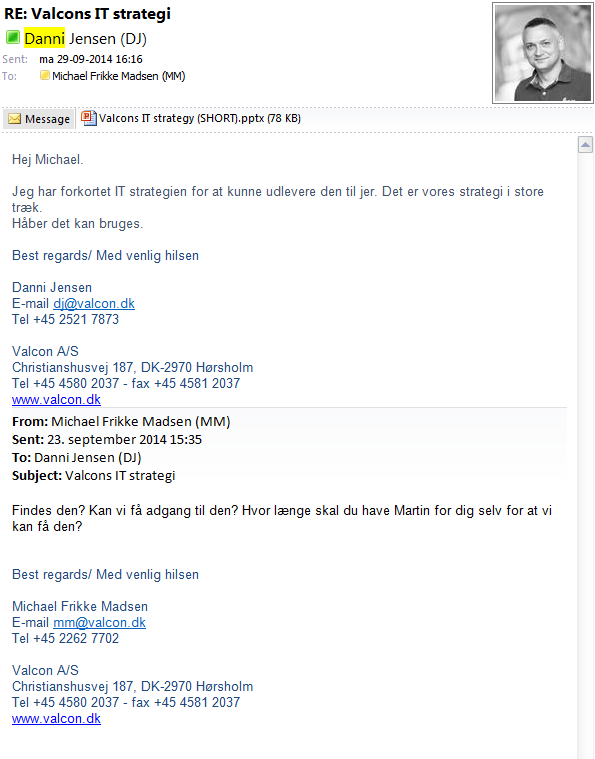
\includegraphics[width=\textwidth]{appendix/danni_communication_1}

\subsection{Valcon Business Strategy}
\label{app:business_strategy_refusal}
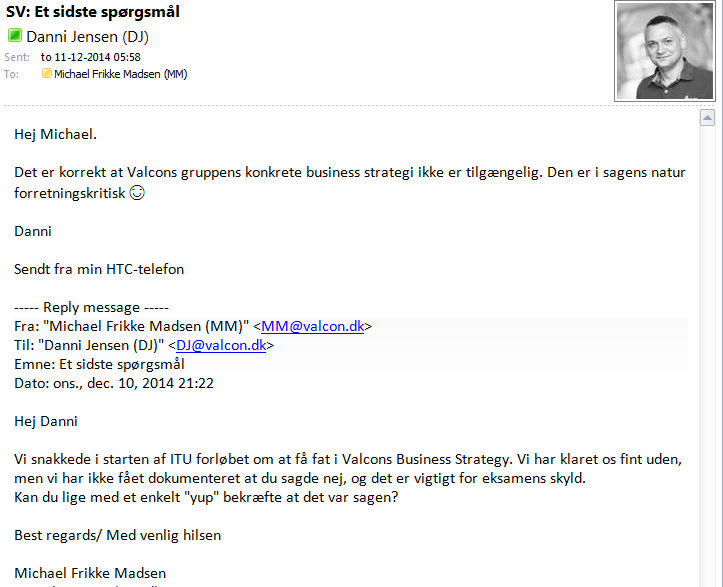
\includegraphics[width=\textwidth]{appendix/danni_communication_2}

It should be noted that we asked for the business strategy early on in process, however this was done verbally, and thus we asked for it again later, to verify that they would not hand it out.

\subsection{Lync conversation 08-09-2014}
Michael Frikke Madsen (MM) [13:02]: 
Du må undskylde at jeg sådan presser på - vi skal bare helst have en bekræftelse på, om vi kan komme ud og holde et introducerende møde inden for de næste par uger, ellers skal vi til at kontakte andre virksomheder for at være sikre på at have noget, når vi reelt skal i gang :) \newline
Danni Jensen (DJ) [13:03]: 
Hej Michael. Det må I gerne, men I kommer selv til at stå for forløbet, forstået på den måde at I selv skal finde interessenter, spørge dem om tid osv
jeg skal selvfølgelig nok sparre med jer, men mit fokus er på Valcon og ikke projektet som sådan. Jeg skal nok komme med mine geniale input når I kommer med noget, men det er jer selv der skal være kreative og opsøgende

\subsection{Lync conversation 17-09-2014}
Michael Frikke Madsen (MM) [12:24]: 
Hey Danni. Vil du/Valcon foretrække dansk eller engelsk til vores rapport?
Vi kan begge dele, men er mest vant til engelsk til rapporter. \newline
Danni Jensen (DJ) [12:35]: 
Engrish pwease \newline
Michael Frikke Madsen (MM) [14:06]: 
Will do (y) \newline
Danni Jensen (DJ) [14:06]: 
Sweet

\subsection{Lync conversation 01-12-2014}
Michael Frikke Madsen (MM) [10:58]: 
Dav Danni
Vi sidder og skriver rapport, og vi skal for eksamens skyld bruge rygdækning til en enkelt ting:
Kan vi snakke/maile med en FO chef, som har erfaring i at ansætte?

Hvis svaret er nej, kan vi roligt skrive i rapporten at det ikke kunne lade sig gøre
Hvis svaret er ja, vil vi skrive en mail med nogle spørgsmål omkring hvad vedkomne ved om ansættelsesprocessen. \newline
Danni Jensen (DJ) [12:47]: 
Hej Michael. Jeg tror det bliver svært at klemme tid ud af en FO chef, de er ikke så gode til at give tid til noget der ikke giver dem opgaver \newline
\linelabel{line:danni_says_no_to_recruiter_interview}
Michael Frikke Madsen (MM) [12:55]: 
Det er i orden - det var også det vi havde gået ud fra, men vi opdagede at vi egentlig ikke havde nogen dokumentation på hvorfor vi ikke havde gjort det 

\section{Communication with Peter}

\subsection{Time Estimation}
\label{app:peter_time_estimation}
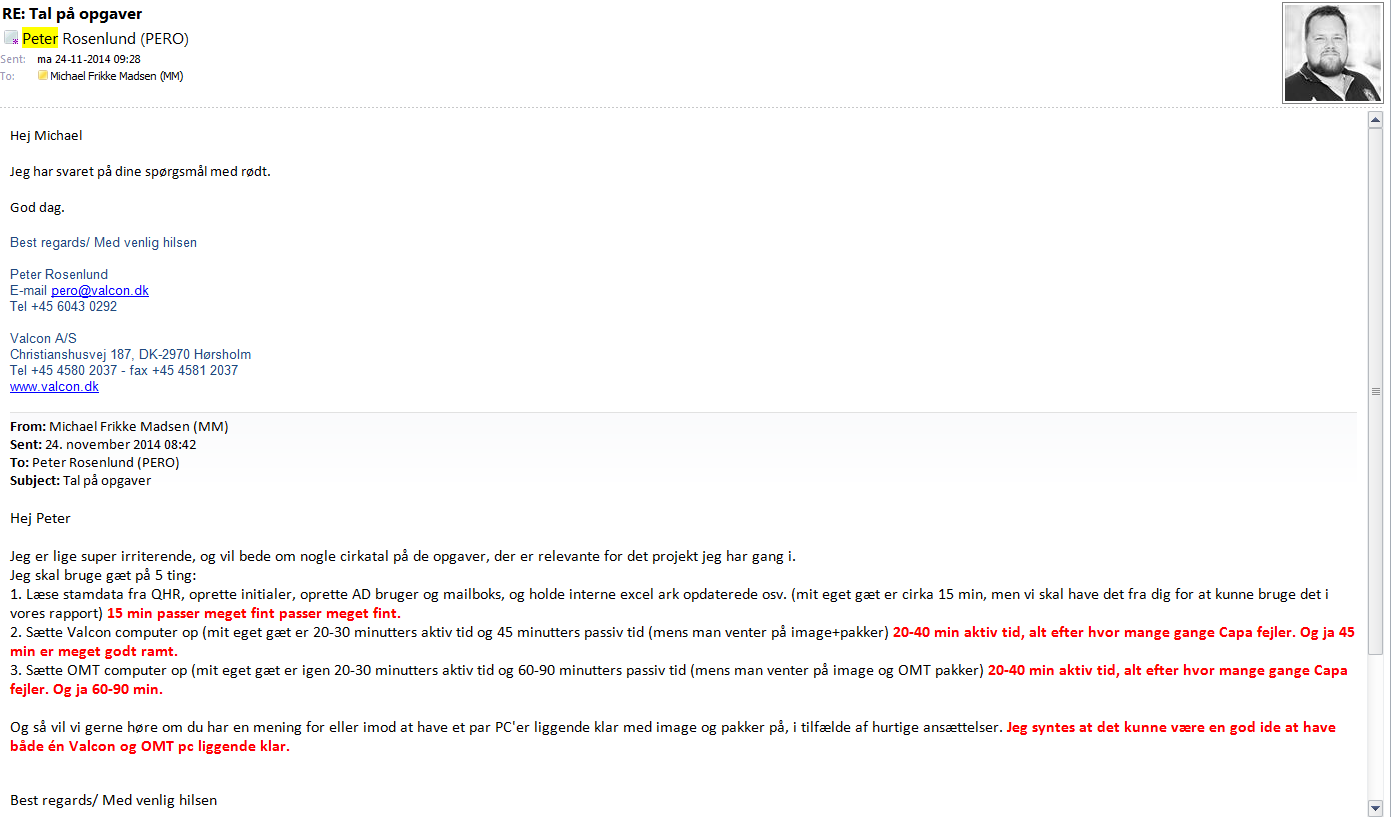
\includegraphics[width=\textwidth]{appendix/peter_communication_1}

\section{Communication with Lisbeth}

\subsection{Time Estimation}
\label{app:lisbeth_time_estimation}
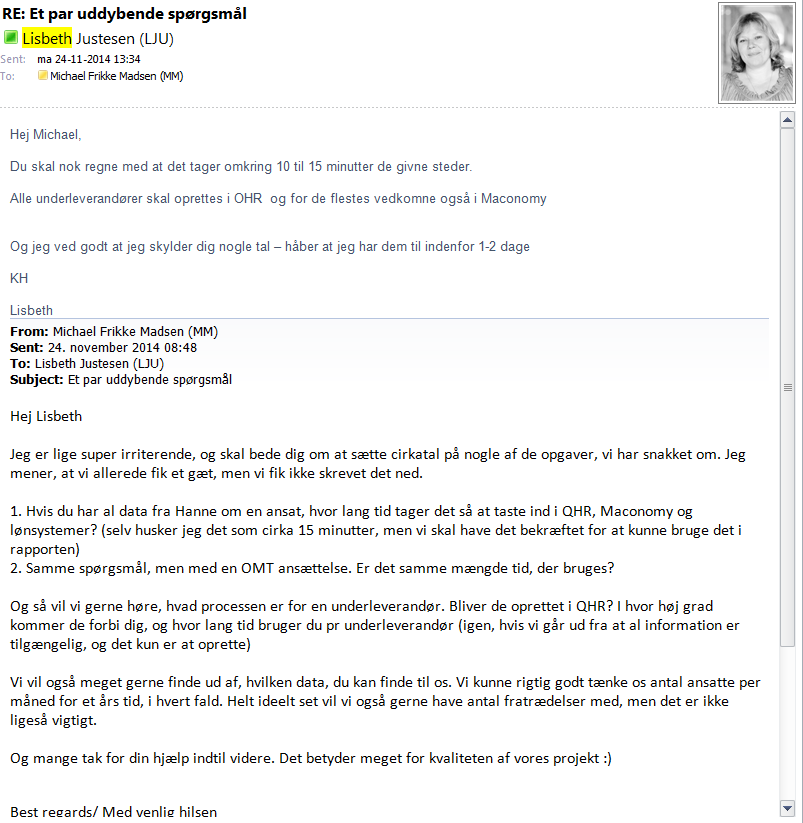
\includegraphics[width=\textwidth]{appendix/lisbeth_communication_1}

\subsection{Data on Hires and Resignations}
\label{app:hires_and_resignations}
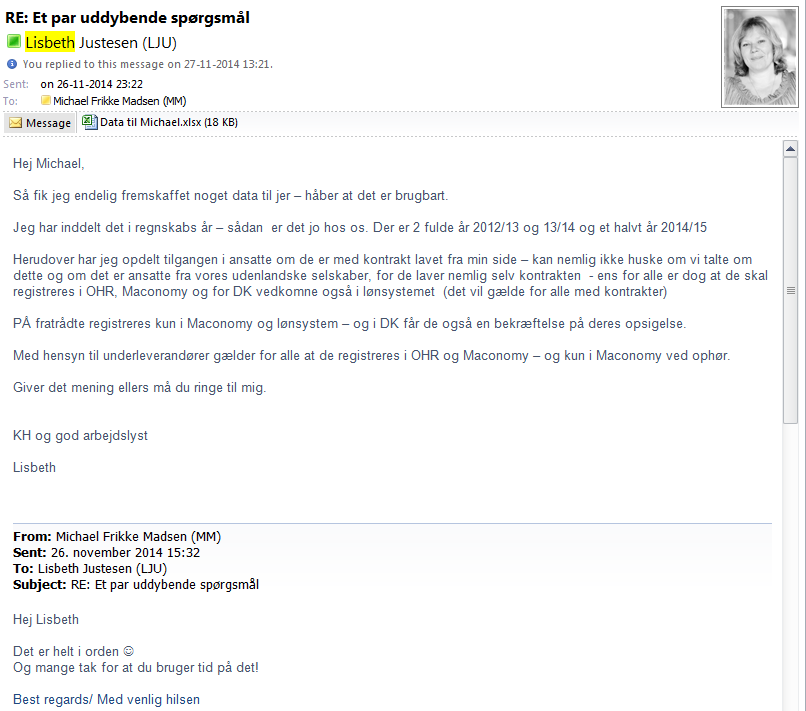
\includegraphics[width=\textwidth]{appendix/lisbeth_communication_2}


\section{Communication with Hanne}

\subsection{Time Estimation}
\label{app:hanne_time_estimation}
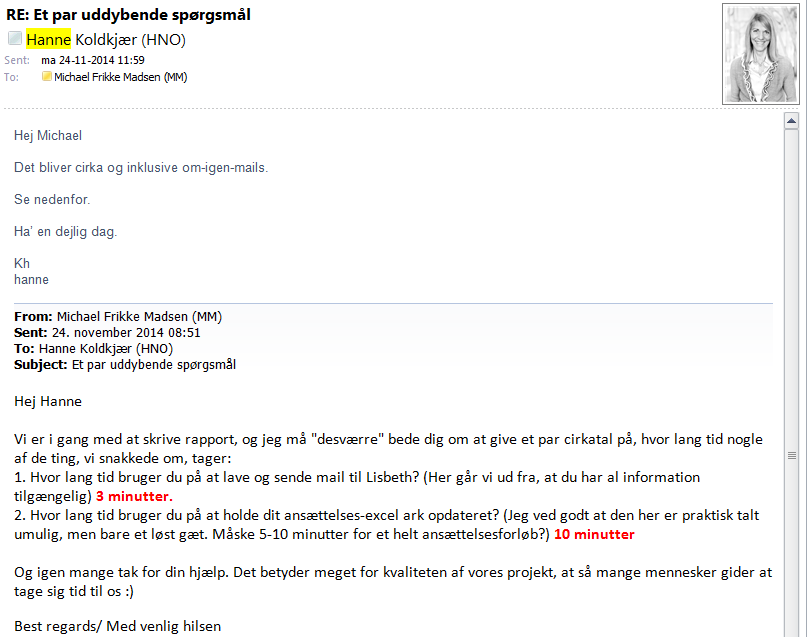
\includegraphics[width=\textwidth]{appendix/hanne_communication_1}


\section{Communication with Jytte}

\subsection{Time Estimation}
\label{app:jytte_time_estimation}
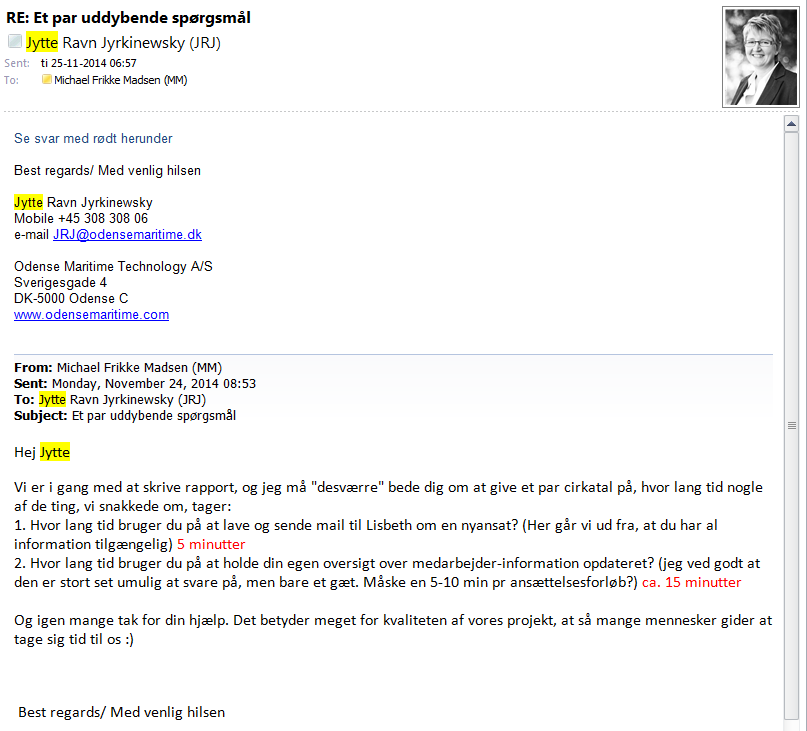
\includegraphics[width=\textwidth]{appendix/jytte_communication_1}

\section{Communication with others}

\subsection{Question to another student help about structure in IT}
\linelabel{matias_on_structure}

\includegraphics[width=\textwidth]{appendix/other_communication_1}
\end{linenumbers*}



\end{document}